% Options for packages loaded elsewhere
\PassOptionsToPackage{unicode}{hyperref}
\PassOptionsToPackage{hyphens}{url}
%
\documentclass[
  abstract]{scrartcl}

\usepackage{amsmath,amssymb}
\usepackage{setspace}
\usepackage{iftex}
\ifPDFTeX
  \usepackage[T1]{fontenc}
  \usepackage[utf8]{inputenc}
  \usepackage{textcomp} % provide euro and other symbols
\else % if luatex or xetex
  \usepackage{unicode-math}
  \defaultfontfeatures{Scale=MatchLowercase}
  \defaultfontfeatures[\rmfamily]{Ligatures=TeX,Scale=1}
\fi
\usepackage{lmodern}
\ifPDFTeX\else  
    % xetex/luatex font selection
\fi
% Use upquote if available, for straight quotes in verbatim environments
\IfFileExists{upquote.sty}{\usepackage{upquote}}{}
\IfFileExists{microtype.sty}{% use microtype if available
  \usepackage[]{microtype}
  \UseMicrotypeSet[protrusion]{basicmath} % disable protrusion for tt fonts
}{}
\makeatletter
\@ifundefined{KOMAClassName}{% if non-KOMA class
  \IfFileExists{parskip.sty}{%
    \usepackage{parskip}
  }{% else
    \setlength{\parindent}{0pt}
    \setlength{\parskip}{6pt plus 2pt minus 1pt}}
}{% if KOMA class
  \KOMAoptions{parskip=half}}
\makeatother
\usepackage{xcolor}
\setlength{\emergencystretch}{3em} % prevent overfull lines
\setcounter{secnumdepth}{5}
% Make \paragraph and \subparagraph free-standing
\makeatletter
\ifx\paragraph\undefined\else
  \let\oldparagraph\paragraph
  \renewcommand{\paragraph}{
    \@ifstar
      \xxxParagraphStar
      \xxxParagraphNoStar
  }
  \newcommand{\xxxParagraphStar}[1]{\oldparagraph*{#1}\mbox{}}
  \newcommand{\xxxParagraphNoStar}[1]{\oldparagraph{#1}\mbox{}}
\fi
\ifx\subparagraph\undefined\else
  \let\oldsubparagraph\subparagraph
  \renewcommand{\subparagraph}{
    \@ifstar
      \xxxSubParagraphStar
      \xxxSubParagraphNoStar
  }
  \newcommand{\xxxSubParagraphStar}[1]{\oldsubparagraph*{#1}\mbox{}}
  \newcommand{\xxxSubParagraphNoStar}[1]{\oldsubparagraph{#1}\mbox{}}
\fi
\makeatother


\providecommand{\tightlist}{%
  \setlength{\itemsep}{0pt}\setlength{\parskip}{0pt}}\usepackage{longtable,booktabs,array}
\usepackage{calc} % for calculating minipage widths
% Correct order of tables after \paragraph or \subparagraph
\usepackage{etoolbox}
\makeatletter
\patchcmd\longtable{\par}{\if@noskipsec\mbox{}\fi\par}{}{}
\makeatother
% Allow footnotes in longtable head/foot
\IfFileExists{footnotehyper.sty}{\usepackage{footnotehyper}}{\usepackage{footnote}}
\makesavenoteenv{longtable}
\usepackage{graphicx}
\makeatletter
\newsavebox\pandoc@box
\newcommand*\pandocbounded[1]{% scales image to fit in text height/width
  \sbox\pandoc@box{#1}%
  \Gscale@div\@tempa{\textheight}{\dimexpr\ht\pandoc@box+\dp\pandoc@box\relax}%
  \Gscale@div\@tempb{\linewidth}{\wd\pandoc@box}%
  \ifdim\@tempb\p@<\@tempa\p@\let\@tempa\@tempb\fi% select the smaller of both
  \ifdim\@tempa\p@<\p@\scalebox{\@tempa}{\usebox\pandoc@box}%
  \else\usebox{\pandoc@box}%
  \fi%
}
% Set default figure placement to htbp
\def\fps@figure{htbp}
\makeatother
% definitions for citeproc citations
\NewDocumentCommand\citeproctext{}{}
\NewDocumentCommand\citeproc{mm}{%
  \begingroup\def\citeproctext{#2}\cite{#1}\endgroup}
\makeatletter
 % allow citations to break across lines
 \let\@cite@ofmt\@firstofone
 % avoid brackets around text for \cite:
 \def\@biblabel#1{}
 \def\@cite#1#2{{#1\if@tempswa , #2\fi}}
\makeatother
\newlength{\cslhangindent}
\setlength{\cslhangindent}{1.5em}
\newlength{\csllabelwidth}
\setlength{\csllabelwidth}{3em}
\newenvironment{CSLReferences}[2] % #1 hanging-indent, #2 entry-spacing
 {\begin{list}{}{%
  \setlength{\itemindent}{0pt}
  \setlength{\leftmargin}{0pt}
  \setlength{\parsep}{0pt}
  % turn on hanging indent if param 1 is 1
  \ifodd #1
   \setlength{\leftmargin}{\cslhangindent}
   \setlength{\itemindent}{-1\cslhangindent}
  \fi
  % set entry spacing
  \setlength{\itemsep}{#2\baselineskip}}}
 {\end{list}}
\usepackage{calc}
\newcommand{\CSLBlock}[1]{\hfill\break\parbox[t]{\linewidth}{\strut\ignorespaces#1\strut}}
\newcommand{\CSLLeftMargin}[1]{\parbox[t]{\csllabelwidth}{\strut#1\strut}}
\newcommand{\CSLRightInline}[1]{\parbox[t]{\linewidth - \csllabelwidth}{\strut#1\strut}}
\newcommand{\CSLIndent}[1]{\hspace{\cslhangindent}#1}

\usepackage{hyperref}
\usepackage{cleveref}
\crefformat{equation}{equation~(#2#1#3)}
\Crefformat{equation}{Equation~(#2#1#3)}
%\renewcommand{\theequation}{\roman{equation}}
%\setkomafont{disposition}{\bfseries}
\usepackage[blocks]{authblk}
%\renewcommand*{\Authsep}{, }
%\renewcommand*{\Authand}{, }
%\renewcommand*{\Authands}{, }
%\renewcommand\Affilfont{\small}
\makeatletter
\patchcmd{\@maketitle}{\LARGE}{\fontsize{14}{17}\selectfont}{}{}
\makeatother
\usepackage[c2]{optidef}
\usepackage{booktabs, longtable, colortbl, array}
\usepackage[flushleft]{threeparttable}
\usepackage{tabularray}
\usepackage[singlelinecheck=false ]{caption}
\Crefformat{table}{Table~(#2#1#3)}
\Crefformat{figure}{Figure~(#2#1#3)} 
\usepackage{float}   
\usepackage[automark]{scrlayer-scrpage}
\usepackage{placeins}
\Crefrangeformat{table}{Tables~(#3#1#4)~to~(#5#2#6)}
\Crefrangeformat{figure}{Figures~(#3#1#4)~to~(#5#2#6)}

\Crefmultiformat{table}{Table~(#2#1#3)}%
{ and~(#2#1#3)}% the second argument is what comes after the first reference
{, (#2#1#3)}% for three or more, separator format
{ and~(#2#1#3)}% for the final reference in a series

\Crefmultiformat{figure}{Figure~(#2#1#3)}%
{ and~(#2#1#3)}% the second argument is what comes after the first reference
{, (#2#1#3)}% for three or more, separator format
{ and~(#2#1#3)}% for the final reference in a series

%\usepackage{fancyhdr}
%\pagestyle{fancy}
%\fancyhead{}
%\fancyhead[RO,LE]{\textbf{Consumer Sentiments}}




%\usepackage[symbol]{footmisc}
\clearpairofpagestyles
%\ohead{\myshorttitle} %running header on right
%\ihead{\myshorttitle} %running header on left
\cfoot*{\pagemark} % Centered page number at the footer
\makeatletter
\@ifpackageloaded{caption}{}{\usepackage{caption}}
\AtBeginDocument{%
\ifdefined\contentsname
  \renewcommand*\contentsname{Table of contents}
\else
  \newcommand\contentsname{Table of contents}
\fi
\ifdefined\listfigurename
  \renewcommand*\listfigurename{List of Figures}
\else
  \newcommand\listfigurename{List of Figures}
\fi
\ifdefined\listtablename
  \renewcommand*\listtablename{List of Tables}
\else
  \newcommand\listtablename{List of Tables}
\fi
\ifdefined\figurename
  \renewcommand*\figurename{Figure}
\else
  \newcommand\figurename{Figure}
\fi
\ifdefined\tablename
  \renewcommand*\tablename{Table}
\else
  \newcommand\tablename{Table}
\fi
}
\@ifpackageloaded{float}{}{\usepackage{float}}
\floatstyle{ruled}
\@ifundefined{c@chapter}{\newfloat{codelisting}{h}{lop}}{\newfloat{codelisting}{h}{lop}[chapter]}
\floatname{codelisting}{Listing}
\newcommand*\listoflistings{\listof{codelisting}{List of Listings}}
\makeatother
\makeatletter
\makeatother
\makeatletter
\@ifpackageloaded{caption}{}{\usepackage{caption}}
\@ifpackageloaded{subcaption}{}{\usepackage{subcaption}}
\makeatother

\usepackage{bookmark}

\IfFileExists{xurl.sty}{\usepackage{xurl}}{} % add URL line breaks if available
\urlstyle{same} % disable monospaced font for URLs
\hypersetup{
  pdftitle={Does Sentiment Predict Consumption Growth of Indian Households?},
  pdfkeywords={Consumption, Consumer Sentiments, Forecasting, Permanent
Income Hypothesis, CPHS},
  hidelinks,
  pdfcreator={LaTeX via pandoc}}


\title{Does Sentiment Predict Consumption Growth of Indian Households?}

%
\author{}

\date{}  % Leaves the date blank if no date is provided

\begin{document}

\maketitle

\begin{abstract}
Leveraging the extensive cross-sectional heterogeneity of the Consumer
Pyramid Household Survey (CPHS) - a comprehensive longitudinal dataset
representative of the Indian economy - this paper investigates the
predictive power of household sentiments on consumption growth through
an Euler equation framework. We select India for our analysis due to its
significantly greater cross-sectional heterogeneity with richer
information content compared to developed countries. We demonstrate that
household sentiments, explained by geographical location, income level,
education attainment, and different demographic characteristics, exhibit
stronger predictive power on consumption growth than raw sentiment
measures themselves. The resulting excess sensitivity of consumption to
sentiments represents a violation of the rational expectations-based
Permanent Income/Life Cycle Hypothesis for Indian households. It
indicates that households' sentiments regarding future financial
positions and business conditions should be appropriately incorporated
when forecasting household consumption, and overall business cycle
dynamics of India. We also argue that, consistent with pre-pandemic
patterns, sentiments should remain crucial for business cycle
forecasting in post-pandemic periods, even though COVID-19 has
fundamentally altered spending patterns and their underlying
determinants for Indian households. Our results broadly parallel
evidence from developed economies, contributing to the broader
literature on sentiment-driven consumption and business cycle
dynamics. %
\\
\\
\noindent%
\textbf{Keywords:} Consumption, Consumer
Sentiments, Forecasting, Permanent Income Hypothesis, CPHS %
 
\vspace{0.5cm}
\noindent%
\textbf{JEL Classification:} E21, E27, C23, C26
\end{abstract}

\pagenumbering{gobble}
\newpage
\pagenumbering{arabic}  
\setcounter{page}{1} 

\setstretch{1.2}
\section{Introduction}\label{sec-1}

Does sentiment predict consumption growth, and if so, why? This question
has rekindled substantial scholarly attention since the advent of
survey-based sentiment data.\footnote{Even before the disaggregated
  micro level sentiments data was available, Acemoglu \& Scott
  (\citeproc{ref-acemoglou1994}{1994}) analyzes the relationship between
  aggregate sentiments, and consumption growth for the UK through the
  Euler equation framework. They find that the evidence of excess
  sensitivity of consumption to sentiments for UK. Using University of
  Michigan's Index of Consumer Sentiments, Carroll et al.
  (\citeproc{ref-carroll_does_1994}{1994}) find that current as well as
  the lagged sentiments positively affect consumption growth even for
  the US.} Our paper examines the predictive power of sentiment on
consumption growth in the context of Indian households, utilizing
longitudinal data from the Consumer Pyramids Household Survey (CPHS).
This paper makes three distinct contributions to the literature. First,
it provides a comprehensive analysis of consumption sensitivity to
sentiment in an emerging market setting, extending the predominantly
developed-market focused literature. Second, it advances the
methodological frontier by developing a novel approach to retain the
cross-sectional heterogeneity and the corresponding information content,
and utilize it in the estimation. Third, it generates new empirical
evidence on how extraordinary economic circumstances - particularly
pandemic-induced uncertainty - influence household spending decisions
and precautionary savings behavior. Our analytical framework, grounded
in the Euler equation, serves dual purposes: it assesses the predictive
capacity of sentiment while simultaneously providing a natural setting
to test for excess sensitivity of consumption to sentiments. This
approach enables us to evaluate the rational expectations-based
Permanent Income/Life Cycle Hypothesis (PIH), which posits that current
consumption fully incorporates all information relevant for predicting
future consumption. Hence, the predictive power of sentiment within the
Euler equation framework directly challenges the prediction of PIH.

Note that the PIH is violated if sentiment predicts consumption growth
within the Euler equation framework. Our paper finds evidence of excess
sensitivity of consumption to sentiment and a violation of the PIH for
Indian households. Moreover, by comparing the OLS estimate of the Euler
equation with that of GMM estimation we show that, instead of the raw
sentiments, the part of the household sentiments explained by the their
geographical location, income, education, and demographics is a much
better predictor of consumption growth of the Indian households. We also
show that, since the Covid-19 pandemic has significant and lasting
impact on the household income risk. It causes changes in the pattern
and the determinants of their spending decisions, and considerably
reduces the predictive capacity of household sentiments falls
significantly in the Covid-periods.

Instead of using the aggregate data, we use disaggregated household
level data because it yields consistent estimates by mitigating
endogeneity concerns stems from the correlation between forecast errors
of consumption and the consumption risk
(\citeproc{ref-Christelis2016}{Christelis et al., 2020};
\citeproc{ref-jappelli2017economics}{Jappelli \& Pistaferri, 2017}).
Complementing this methodological insight, Lahiri \& Zhao
(\citeproc{ref-lahiri_determinants_2016}{2016}) argue that household
sentiment transcends mere reflections of aggregate macroeconomic
conditions, and it encapsulates substantial idiosyncratic information
shaped by households' subjective interpretations of aggregate economic
conditions. Arguments of the extant literature posited above underscore
the importance of preserving and appropriately leveraging the rich
information embedded in micro-level sentiment data - particularly its
time-varying cross-sectional heterogeneity - when forecasting
consumption patterns.\footnote{Toussaint-Comeau \& McGranahan
  (\citeproc{ref-toussaint2006variations}{2006}), Dominitz \& Manski
  (\citeproc{ref-dominitz2004should}{2004}), and Lahiri et al.
  (\citeproc{ref-lahiri_forecasting_2016}{2016}) also advocate to use
  the disaggregated level data as due to its rich information content,
  which enhances the informative and predictive power of the sentiment
  index.}

Realizing the potential benefits of the micro level survey data,
Christelis et al. (\citeproc{ref-Christelis2016}{2020}) employs
survey-based estimates of consumption growth and risk to calculate the
index of prudence and examine precautionary savings for Netherlands
through the Euler equation framework. Building on this approach,
Immordino et al. (\citeproc{ref-immordino2024consumption}{2024})
investigates household spending decisions during the COVID-19 pandemic
using data from 3,016 Italian households. They find a positive
relationship between the expected consumption growth, and the expected
disposable income growth, but did not find any significant relationship
between income risk and the expected consumption growth in their
analysis. Surprisingly, health factors did not emerge as primary drivers
of Italian household spending decisions during the pandemic.
Additionally, Pistaferri (\citeproc{ref-pistaferri2016}{2016})
demonstrates that consumer confidence, alongside the leverage ratios
significantly explains the sluggish recovery of U.S. consumption
following the Great Recession. Souleles
(\citeproc{ref-souleles_expectations_2004}{2004}) on the other hand,
investigates the excess sensitivity of consumption to sentiments through
the Euler equation framework by using the household level data of the
US. His methodology involved matching consumption data from the Consumer
Expenditure Survey (CEX) with sentiment data underlying Michigan's Index
of Consumer Sentiment (ICS) through demographic characteristics. As a
result, Souleles (\citeproc{ref-souleles_expectations_2004}{2004})
applies two-sample IV estimation method of Angrist \& Krueger
(\citeproc{ref-angrist_effect_1992}{1992}) to ensure appropriate
standard errors and valid statistical inference. While finding evidence
of excess sensitivity and PIH violation for U.S. households, Souleles
(\citeproc{ref-souleles_expectations_2004}{2004}) uniquely documents a
negative relationship between household-level sentiments and consumption
growth.

Against this backdrop, our paper investigates whether sentiments predict
consumption growth for Indian households. We use the Euler equation
framework provides for our analysis which provides a natural setting to
examine both consumption's excess sensitivity to sentiments and the
validity of the PIH in the Indian context. This study represents the
first comprehensive examination of household sentiment's predictive
capacity and consumption excess sensitivity for Indian
households\footnote{Priya \& Sharma
  (\citeproc{ref-priya_sharma2024}{2024}) have used the data of
  sentiments of Indian households to estimate a consumption function.
  Their primary objective was to test the role of animal spirits in the
  propagation of the oil price and the monetary policy shock for the
  Indian economy.}. We select India for our analysis due to its
significantly greater cross-sectional heterogeneity and hence the richer
information content compared to developed economies. However, accurately
estimating sentiment's predictive power requires preserving the
substantial cross-sectional heterogeneity within Indian data, which
contains valuable information as emphasized by Lahiri \& Zhao
(\citeproc{ref-lahiri_determinants_2016}{2016}).

The cross-sectional heterogeneity in household real consumption growth
stems from two sources: variation in nominal consumption expenditure and
household-specific inflation rates. Prior literature has typically
overlooked this latter source of heterogeneity by using aggregate CPI to
deflate nominal consumption, which lacks cross-sectional variation.
Consequently, real consumption growth calculations based on aggregate
CPI capture only partial cross-sectional heterogeneity---specifically,
the variation in nominal consumption while neglecting differences in
household-specific inflation experiences. To preserve the complete
cross-sectional heterogeneity, we derive an expenditure-minimizing
consumption bundle for Indian households. This approach, which deflates
nominal consumption by household-specific price indices, fully maintains
the time-varying cross-sectional heterogeneity in real consumption. We
employ this expenditure-minimizing consumption bundle as our measure of
real consumption throughout our analysis\footnote{Similarly, we
  calculate real household specific real income by deflating their
  nominal income using the corresponding household specific price
  indices to preserve the true cross-sectional heterogeneity of
  household specific real income.}. Given that food and fuel \& lighting
constitute approximately 92\% of Indian household expenditures, we
construct two expenditure-minimizing consumption bundles: (1) a food
bundle comprising 8 major food groups, and (2) a food \& fuel bundle
that incorporates fuel \& lighting alongside these food groups. These
bundles serve as our real consumption measures.

We use both OLS, and GMM to estimate the Euler equation for the period
April, 2016 to October 2022. We employ two distinct sentiment measures:
households' perceptions of their future financial position and their
expectations regarding future business conditions. In the OLS
estimation, we use the raw sentiments of the households as the control
variable that takes three discrete values -- 1, 0, and -1. The
coefficient of the sentiments obtained from OLS indicates the proportion
of the variance of consumption growth of Indian households can be
explained by their raw sentiments. It is important to mention here that,
Blendon et al. (\citeproc{ref-blendon1997}{1997}) argues that
individuals form their sentiments mostly by processing information
obtained during the conversation with their neighbors at the backyard of
their house. Following this insight and Souleles
(\citeproc{ref-souleles_expectations_2004}{2004}), we implement GMM
estimation using geographical location, income level, educational
attainment, and other demographic characteristics as instruments for
household sentiment. This approach enables us to assess whether the part
of sentiment explained by these socioeconomic factors provides superior
predictive power compared to raw sentiment measures. We find that the
part of the household sentiments explained by their geographical
location, income, education, and demographics is a superior predictor of
their consumption growth than the raw sentiments itself. Our results
reported in {Table~\ref{tbl-gmm_combined}} also show that, the fuel
consumption of Indian households is more sensitive to their sentiments
than the food consumption.

Moreover, we estimate our model separately for the pre-COVID period
(April 2016-February 2020) and the COVID period (March 2020-October
2022) to examine the COVID-19 pandemic's impact on household spending
decisions. We find that only expectations regarding households' own
future financial position predict food bundle consumption growth.
However, for the combined food \& fuel bundle, both personal financial
expectations and business condition sentiments predict consumption
growth, with the latter demonstrating superior predictive power.
Notably, sentiment's predictive capacity diminishes substantially during
the COVID period. Our results further reveal that the COVID-19 pandemic
has exerted lasting effects on job prospects, health, and income risk.
In the absence of comprehensive social security systems, these effects
have fundamentally altered both spending patterns and their determinants
among Indian households, as evidenced by the reduced predictive power of
sentiment during this period. To address potential spurious excess
sensitivity, we incorporate household forecast errors as a control
variable in our estimation, following Souleles (2004). The results
remain qualitatively identical to specifications without systematic
control for forecast errors, confirming the robustness of our findings.
The results of our paper broadly parallel evidence from developed
economies, contributing to the broader literature on sentiment-driven
consumption and business cycle dynamics.\footnote{See, Vuchelen
  (\citeproc{ref-vuchelen2004consumer}{2004}) and references therein for
  a comprehensive analysis on sentiment and business cycle.}

The rest of the paper proceeds as follows. Section~\ref{sec-2} describes
the data, and Section~\ref{sec-3} briefly discusses the PIH and the
excess sensitivity of consumption. Section~\ref{sec-4} presents the
results, and Section~\ref{sec-5} concludes.

\section{Data Description}\label{sec-2}

We collect data of household sentiments from Consumer Pyramid Household
Survey (CPHS).\footnote{The Consumer Pyramid Household Survey (CPHS) is
  conducted thrice every year since 2014 by the Centre for Monitoring
  Indian Economy (CMIE). Under CPHS, a large panel of sample households
  are surveyed under CPHS to measure the household well-being in India.
  This large longitudinal dataset is widely acknowledged as
  representative of the Indian economy. For details see;
  \url{https://consumerpyramidsdx.cmie.com/}} It is a large longitudinal
data set, representative of Indian economy. CPHS collects data of
household sentiments of India since April, 2016. To collect the
sentiment data, a generic Indian household h is surveyed thrice in a
year, e.g.; a household surveyed in April, 2016 is surveyed again in
August, 2016 by CPHS for the collection of the sentiments data and so
on. To assess the sentiments, CPHS asks questions about the present
conditions as well as the future expectations of the household financial
position, and the business condition. In the process, to assess the
present conditions, CPHS asks the following 2 questions to the
households - (I) Compared to a year ago, how is your family faring
financially these days?; and (II) Do you think that this is generally a
good or bad times to buy things like furniture, refrigerator,
television, two-wheeler, and car? Along with this, CPHS asks the
following 3 questions to assess the short-run and the long-run future
expectations of the households - (III) How do you think that a year from
now, financially, your family would be faring?; (IV) How would you
describe the financial and business conditions in our country in the
next 12 months?; and (V) What do you think would be the financial and
business conditions in our country in the next 5 years? The answer to
questions (I), and (III) are recorded as Better, Same and Worse, and
accordingly a numerical value, 1, 0, -1 is assigned. On the other hand,
answers to questions (II), (IV) and (V) are recorded as Good time,
uncertain time and Bad time, and accordingly a numerical value, 1, 0 and
-1 is assigned to the answer.

Along with sentiments, we also collect data of household's monthly
expenditure on 8 major food groups, and fuel \& lighting from CPHS from
April 2016. The 8 major food groups include - (1) cereals; (2) oils and
fats; (3) fruits; (4) pulses and products; and (5) milk and milk
products; (6) meat, fish and egg; (7) vegetables and spices; and (8)
sweets and snacks. Along with the above mentioned 8 food groups, we also
collect data on household expenditure share for food \& fuel. We find
that the 8 food groups and the fuel and lightning contribute almost 92\%
of the expenditure for the Indian households. Table~\ref{tbl-desc}
reports the descriptive statistics of the data collected from CPHS.
Using this data, and by using the methodology described below, we
calculate two types of expenditure minimizing consumption bundles for
the Indian households -- (i) food bundle: consisting of the 8 food
groups mentioned above; and (ii) food \& fuel bundle: consisting of the
fuel \& lighting along with the 8 food groups mentioned above.

\begin{table}

\caption{\label{tbl-desc}Descriptive Statistics}

\centering{

    \centering
     % Overall table caption
    

    \small % Reduce font size

    % Subtable 1 caption
    \caption*{(a): Demographic Variables} 

    % First Subtable: Table 1(a)
    \begin{subtable}{\textwidth}
    \label{tbl-des_a}
        \centering
        \renewcommand{\arraystretch}{0.9}
        \begin{tabular}{p{5cm} c}
            \toprule
            \textbf{Variable} & \textbf{Mean/Proportion} \\ 
            \midrule
            \textbf{Income} & 19,834.12 \\ 
            \textbf{Age} & 46.34 \\ 
            \addlinespace
            \textbf{Education} & \\ 
            \quad Less than 5 & 27.5 \\ 
            \quad 5-10 & 56.4 \\ 
            \quad 10-12 & 8.7 \\ 
            \quad 13-15 & 7.0 \\ 
            \quad 15+ & 0.4 \\ 
            \addlinespace
            \textbf{Gender} & \\ 
            \quad Male & 88 \\ 
            \quad Female & 12 \\ 
            \addlinespace
            \textbf{Marital Status} & \\ 
            \quad Married & 85 \\ 
            \quad Unmarried & 15 \\ 
            \addlinespace
            \textbf{Geographic Location} & \\ 
            \quad Rural & 25 \\ 
            \quad Urban & 75 \\ 
            \addlinespace
            \textbf{Occupation} & \\ 
            \quad Agriculture and Allied & 15.4 \\ 
            \quad Manufacturing, Industry and Auto & 34.1 \\ 
            \quad Services, Media, Health & 50.3 \\ 
            \quad Others & 0.2 \\ 
            \bottomrule
        \end{tabular}
        \label{tbl-desc-a}
    \end{subtable}

    \vspace{1.5em} % Add some vertical space between subtables

    % Subtable 2 caption
    \caption*{(b): Sentiment Variables} 

    % Second Subtable: Table 1(b)
    \begin{subtable}{\textwidth}
    \label{tbl-des_b}
        \centering
        \renewcommand{\arraystretch}{0.9}
        \begin{tabular}{p{3cm} p{2cm} c c c c c c}
            \toprule
            \textbf{Variable} & \textbf{Response} & \multicolumn{2}{c}{\textbf{Full Sample}} & \multicolumn{2}{c}{\textbf{Pre-Covid}} & \multicolumn{2}{c}{\textbf{Covid}} \\ 
            \cmidrule(lr){3-4} \cmidrule(lr){5-6} \cmidrule(lr){7-8}
            & & \textbf{N} & \textbf{\%} & \textbf{N} & \textbf{\%} & \textbf{N} & \textbf{\%} \\ 
            \midrule
            QFP & Bad & 12,610 & 21.4 & 5,097 & 12.9 & 7,513 & 38.8 \\ 
                & Same & 34,245 & 58.2 & 24,010 & 60.8 & 10,235 & 52.9 \\ 
                & Good & 12,016 & 20.4 & 10,407 & 26.3 & 1,609 & 8.3 \\ 
            \addlinespace
            QBC & Bad & 13,671 & 23.2 & 5,544 & 14.0 & 8,127 & 42.0 \\ 
                & Same & 30,628 & 52.0 & 20,894 & 52.9 & 9,734 & 50.3 \\ 
                & Good & 14,572 & 24.8 & 13,076 & 33.1 & 1,496 & 7.7 \\ 
            \midrule
            \multicolumn{2}{l}{Total N} & 58,871 & & 39,514 & & 19,357 & \\ 
            \bottomrule
        \end{tabular}
        \label{tbl-desc-b}
    \end{subtable}

}

\end{table}%

Along with this, we also collect data on the price index of the
aforementioned eight food groups, as well as fuel and lighting, from
MoSPI\footnote{See; \href{https://mospi.gov.in/}{mospi.gov.in} for the
  data of price index.}. MoSPI directly reports the price index for the
first five food groups---(1) to (5) listed above. However, it separately
provides the price index for the following food items:(i) Meat and fish
(ii) Egg (iii) Vegetables (iv) Spices (v) Sweets (vi) SnacksUsing the
price indices of these food items and their corresponding weights, we
calculate the monthly price index for the remaining three food
groups:(6) Meat, fish, and eggs (7) Vegetables and spices (8) Sweets and
snacks

\section{The PIH and the Excess Sensitivity of Consumption -- The
Model}\label{sec-3}

Suppose, a generic household \(h\), belonging to the geographical
location \(j\) calculates the minimum expenditure required to obtain a
certain amount of consumption bundle by solving the following static
problem in each period \(t\),

\begin{mini*}|l|
{}{e_{h, t}^j=\sum_{i=1} p_{i, t}^j c_{i, h t}^j \,; \quad h=1,2,\ldots,H; \quad j={\ rural,urban\ }}
{}{}
\addConstraint{c_{h,t}^j}{=}{\prod_{i=1}^{n}\left(c_{i,ht}^j\right)^{a_{i,ht}^j} \,;\quad \sum_{i=1}^{n}{\alpha_{i,ht}^j=1;}}
\end{mini*}

where, \(p_{i,t}^j\) is the price of the \(i^{th}\) sub-category of
consumption at, time \(t\) for the household, \(h\) located at the
\(j^{th}\) geographical area. \(c_{i,h,t}^j\), and \(\alpha_{i,h,t}^j\)
are the real respectively the demand, and the expenditure share of the
\(i^{th}\) sub-category of goods by household, \(h\); belonging to the
\(j^{th}\) geographical location at \(t\). \(e_{h,t}^j\) is the nominal
expenditure of household, \(h\); belonging to the \(j^{th}\)
geographical location at time, \(t\). The optimization yields an
expenditure minimizing consumption bundle for the household, \(h\);
located at the \(j^{th}\) geographical location at time, \(t\), as
written as written in Equation~\ref{eq-basket}. It is a measure of real
consumption of the household, \(h\) located at the \(j^{th}\)
geographical area at time, \(t\). We use real consumption, and
consumption synonymously in this paper.

\begin{equation}\phantomsection\label{eq-basket}{
c_{h,t}^j=\frac{k_{h,t}^j\ e_{i,h,t}^j}{p_{h,t}^j}
}\end{equation}

where, \(p_{h,t}^j\) is a measure of aggregate price index for household
\(h\), belonging to the \(j^{th}\) geographical location at \(t\) as
written below,

\begin{equation}\phantomsection\label{eq-price}{ 
p_{h,t}^j=\prod_{i=1}^{n}\left(p_{i,t}^j\right)^{\alpha_{i,ht}^j}\ ;
}\end{equation}

and,

\[
k_{h,t}^j=\prod_{i=1}^{n}{\alpha_{i,ht}^j}^{\alpha_{i,ht}^j}
\]

Next, the generic household \(h\) solves an intertemporal problem to
decide the time path of consumption.

\begin{maxi*}|l|
    {}{E_0\sum_{t=0}^{\infty}\beta^t \log\left(c_{h,t}^j\right)}{\label{eq:objective}}{}
    \addConstraint{a_{h,t}^j - c_{h,t}^j}{= \frac{a_{h,t+1}^j}{R_{t+1}}}{}
    \addConstraint{
        \begin{aligned}
        a_{h,0}^j &= \text{given} \quad &\text{(Initial condition)} \\
        \lim_{t \to \infty} R^{-(t+T)}a_{h,t}^j &\geq 0 \quad &\text{(Transversality Condition (TVC))}
        \end{aligned}
    }{}
\end{maxi*}

where, \(a_{h,t}^j\) is the real income, of household \(h\), belonging
to the \(j^{th}\) geographical location at \(t\), \(R_{t}\)is the gross
real interest rate at time, \(t\), and \(0<\beta<1\) is the discount
factor. Under logarithmic utility function, and \(\beta=R^{(-1)}\), the
Euler equation gives

\begin{equation}\phantomsection\label{eq-euler}{
\Delta ln(c_h(t+1)^j\ )=\delta_{h(t+1)}^j
}\end{equation}

where, \(E_t\left(\delta_{h\left(t+1\right)}^j\right)=0\).
Equation~\ref{eq-euler} implies the absence of excess sensitivity of
consumption -- factors included in the information set of the households
at \(t^{th}\) period cannot forecast the consumption growth of the (t+1)
period. Note, the absence of excess sensitivity of consumption implies
that the current consumption contains all the relevant information to
forecast future consumption. Note,
\(E_t\left(\delta_{h\left(t+1\right)}^j\right)=0\ \Rightarrow E_t\left(\Delta ln\left(c_{h\left(t+1\right)}^j\right)\right)=E\left(\Delta ln\left(c_{h\left(t+1\right)}^j\right)\middle| I_{ht}^j\right)=0;\)
where, \(I_{ht}^j\) is the information set of household h belonging to
the location \(j\) at the \(t^{th}\) period. This yields,
\(E_t\left(ln\left(c_{h\left(t+1\right)}^j\right)\right)=ln\left(c_{ht}^j\right)\),
implying current consumption contains all the relevant information to
forecast future consumption. Suppose, \(x_{ht}^j\in I_{ht}^j\) but,
\(x_{ht}^j\neq c_{ht}^j\). The PIH implies that, \(x_{ht}^j\) cannot
predict, \(c_{h\left(t+1\right)}^j\). If \(x_{ht}^j\) predicts
\(c_{h\left(t+1\right)}^j\), the excess sensitivity of consumption to
\(x_{ht}^j\) exists, and the PIH is violated.\footnote{Therefore, to
  test the excess the excess sensitivity of consumption to \(x_{ht}^j\),
  we include \(x_{ht}^j\) in the Euler equation as one of the control
  variables, and test the significance of its estimated coefficient
  (see, {Equation~\ref{eq-sol1} and Equation~\ref{eq-sol2}} in the
  text). A significant estimated coefficient of \(x_{ht}^j\) implies the
  presence of excess sensitivity of consumption to \(x_{ht}^j\), and the
  violation of PIH (\citeproc{ref-hall1978}{Hall, 1978};
  \citeproc{ref-jappelli2017economics}{Jappelli \& Pistaferri, 2017}).}

\subsection{The Time-varying Cross-sectional
Heterogeneity}\label{sec-3.1}

Extant literature calculates the household specific real consumption by
deflating their nominal consumption through the aggregate CPI. Since,
aggregate CPI only changes with time, and does not change across
households; such a measure of real consumption only partially captures
the cross sectional heterogeneity of the real consumption. It leads to
the loss of potentially rich information content of the data especially
for a country like India with a vast cross-sectional
heterogeneity\footnote{The relative importance of different commodities
  in the consumption basket varies over time, and across individuals
  belonging to the different socioeconomic strata of the society. As a
  result, the incidence of inflation also varies across individuals and
  over time. Ignoring the changing relative importance of different
  commodities for different groups of people yields a Plutocratic bias
  of the CPI (\citeproc{ref-nachane2019plutocratic}{Nachane \& Chaubal,
  2019}). A disaggregated household specific price level can address the
  Plutocratic bias associated with aggregate price index.}. To
comprehend the information loss, we calculate the household specific
price index from Equation~\ref{eq-price} using the monthly data of CPI
for the food bundle, and food \& fuel bundle. Consequently, we calculate
the household specific y-o-y inflation rate for food bundle, and food \&
fuel bundle as follows -

\[
\pi_{h(t+1)}^j=\ln \left(p_{h,(t+1)}^j\right)-\ln \left(p_{h,(t+1)-12)}^j\right)
\]

Next, we classify the households in 4 categories according to the
occupation of their household heads, calculate the average inflation
rate from May 2017 to October 2022, and plot them in
Figure~\ref{fig-mean_occup}. Alongside the average inflation rate,
Figure~\ref{fig-mean_occup} also plots the average inflation rate based
on the aggregate CPI. While the upper panel of
Figure~\ref{fig-mean_occup} plots the average inflation rates for the
food bundle, the lower panel depicts the average inflations for the food
\& fuel bundle. Figure~\ref{fig-mean_occup} shows that, the average
inflation rate significantly varies across different types of households
and also over time.

\begin{figure}

\centering{

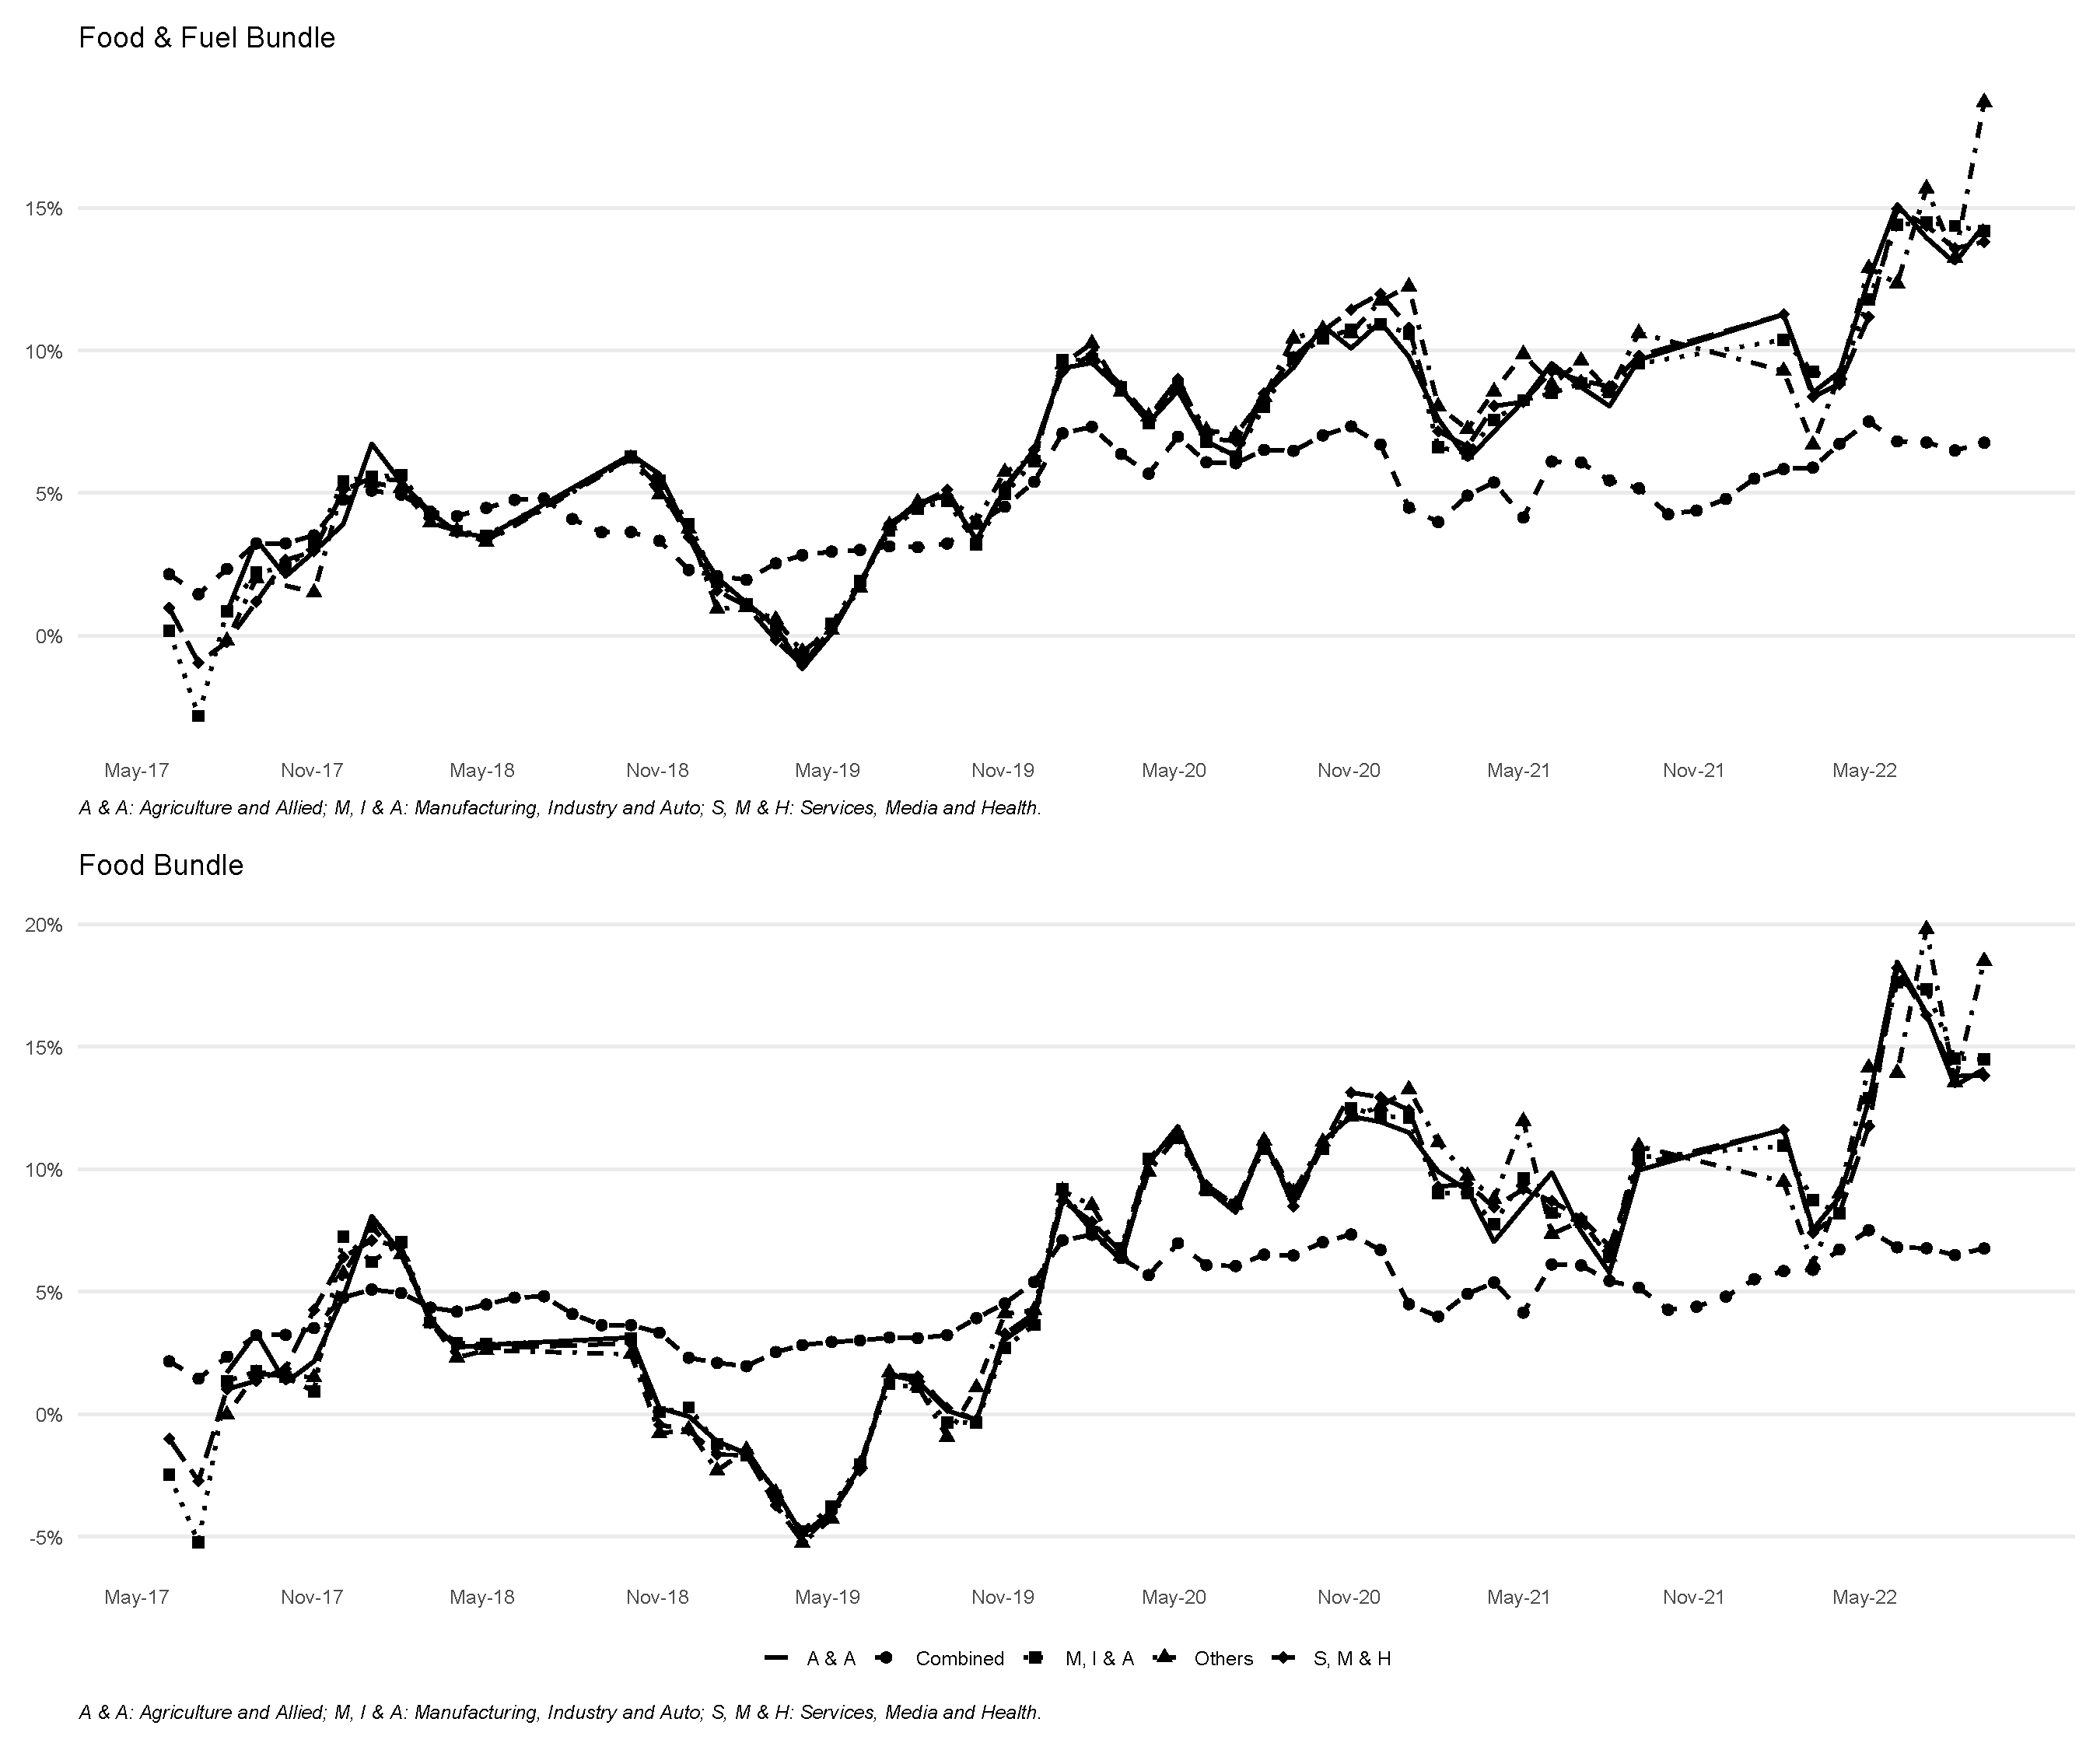
\includegraphics[width=\linewidth,height=1.5\textheight,keepaspectratio]{images/mean_occupation_cat_Phmt.pdf}

}

\caption{\label{fig-mean_occup}Cross-sectional Heterogeneity of Average
Aggregate Inflation Rate, and Household Specific Inflation Rate -
Households Classified in terms of Occupations of Household Head}

\end{figure}%

Since, households often change occupation over time, we calculate the
inflation rate after classifying the households according to the
educational qualification, and the age of the household head.
{Figure~\ref{fig-mean_educ} and Figure~\ref{fig-mean_age}} (see appendix
for figures) plot the average inflation rate from May 2017 to October
2022 for the Indian households classified according to the educational
qualification, and the age of the household head respectively. Like
Figure~\ref{fig-mean_occup}, {Figure~\ref{fig-mean_educ} and
Figure~\ref{fig-mean_age}} also portray the significant variation of the
average inflation rate across different types of households

Next, to understand the cross-sectional heterogeneity in real
consumption, we calculate a monthly household-specific
expenditure-minimizing consumption bundle for food bundle, and for food
\& fuel bundle using Equation~\ref{eq-basket}. The
expenditure-minimizing consumption bundles represent the
household-specific real consumption in our paper. Note, such a measure
of real consumption of the households incorporates the time-varying
cross-sectional heterogeneity of both nominal consumption, and the price
level, and thereby fully preserves the information content of the data
relevant for forecasting (\citeproc{ref-lahiri_determinants_2016}{Lahiri
\& Zhao, 2016}).

Using the measure of real consumption described above, we calculate its
growth rate as follows:

\[
\Delta \ln \left(c_{h(t+1)}^j\right)=\Delta \ln \left(e_{h(t+1)}^j\right)+\Delta \ln \left(k_{h(t+1)}^j\right)-\pi_{h(t+1)}^j
\]

To understand the cross-sectional heterogeneity of consumption, we plot
the average real consumption growth for the 4 categories of households,
classifieds according to the occupation of their household head in
Figure~\ref{fig-mean_occup_chmt}. Along with the disaggregated level of
consumption expenditure for different types of households,
Figure~\ref{fig-mean_occup_chmt} also plots the average aggregate real
consumption growth for all the households. While the upper panel of
Figure~\ref{fig-mean_occup_chmt} plots the average consumption growth
for the food bundle, the lower panel depicts the same for the food \&
fuel bundle. Figure~\ref{fig-mean_occup_chmt} shows- (i) the significant
variation in consumption growth across the five types of households, and
also over time, and (ii) the reduction in the average consumption growth
for all types of households due to the Covid-19 pandemic.
Figure~\ref{fig-mean_occup_chmt} also shows the slow recovery of the
consumption of Indian households in the periods after the Covid-19
pandemic.

{Figure~\ref{fig-mean_educ_chmt} and Figure~\ref{fig-mean_age_chmt}} on
the other hand, portray the average consumption growth from May 2017 to
October 2022 when the households are classified according to the
educational qualification, and the age of the household head.
{Figure~\ref{fig-mean_educ_chmt} and Figure~\ref{fig-mean_age_chmt}}(see
appendix for figures) also depict significant time-varying cross
sectional heterogeneity, and the slow recovery of the consumption growth
from the Covid-19 pandemic shock for the Indian households. The
significant time-varying cross sectional heterogeneity depicted in
{Figure~\ref{fig-mean_occup_chmt} to Figure~\ref{fig-mean_age_chmt}}
show that, the average consumption growth for the Indian households has
a definite pattern, and it is not random as predicted by the PIH as
mentioned above in Equation~\ref{eq-euler}. Note in our expenditure
minimizing consumption bundle, the time-varying cross-sectional
heterogeneity of real consumption arises from the time-varying
cross-sectional heterogeneity of the nominal consumption, and the
household specific price level. Therefore, the expenditure minimizing
consumption bundle used by us as a measure of real consumption, fully
preserves the information content arising from the cross-sectional
heterogeneity in household specific nominal consumption, and the
household specific price level, which is relevant for better forecasting
(\citeproc{ref-lahiri_determinants_2016}{Lahiri \& Zhao, 2016}).

\begin{figure}

\centering{

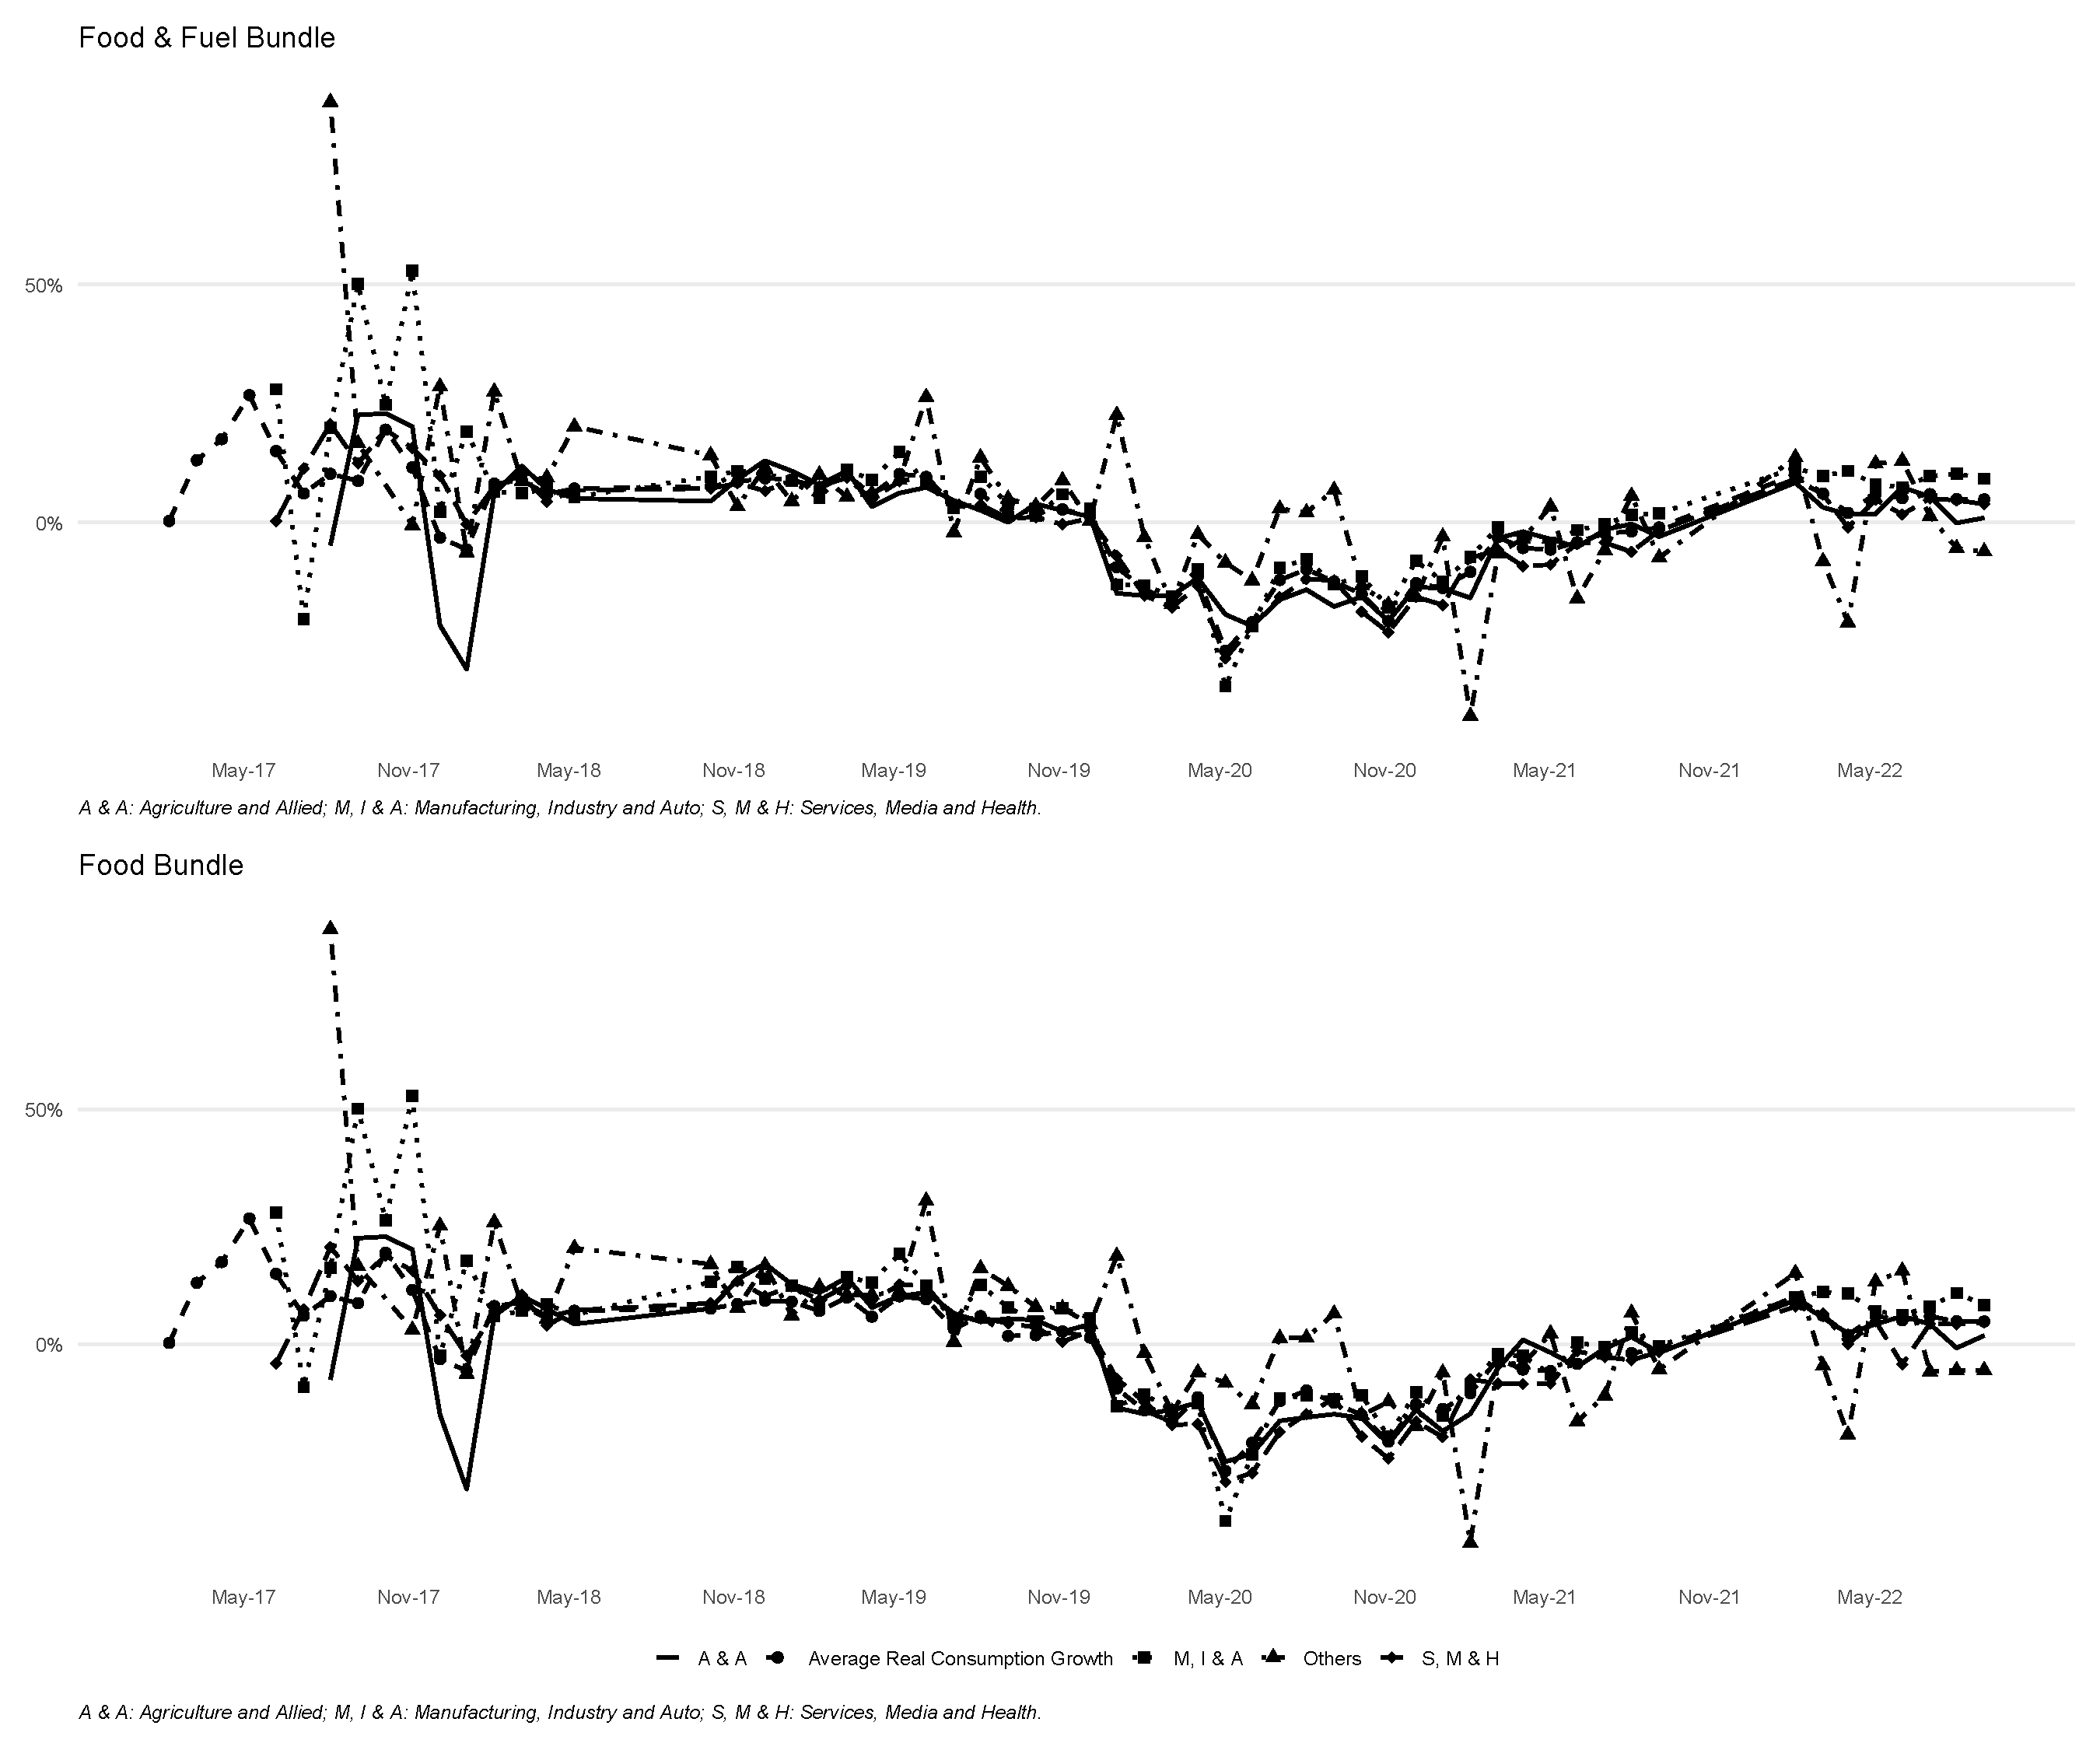
\includegraphics[width=\linewidth,height=1.5\textheight,keepaspectratio]{images/mean_occupation_cat_Chmt.pdf}

}

\caption{\label{fig-mean_occup_chmt}Cross-sectional Heterogeneity of
Household Specific Consumption Growth - Households Classified in terms
of Occupation of Household Head}

\end{figure}%

\section{Does Sentiment Predict Consumption Growth?}\label{sec-4}

This section examines the relationship between the aggregate consumption
growth, and the aggregate sentiments for India from May 2017 to October
2022. To do so, we calculate an Index of Consumer Sentiments (ICS) for
India using the average of the balance statistics of the sentiments
associated with -- (i) the year ahead household's own future financial
positions (question III of CPHS), and (ii) the overall business
condition of the economy (question IV of CPHS). The balance statistics
of sentiments is calculated by adding 100 with the difference between
the proportion of optimistic respondents and the pessimistic respondents
for a given question. Note, when the proportion of optimistic
respondents equals the proportion of the pessimistic household, the
balance statistics of sentiments takes its baseline value 100.
Similarly, when the proportion of optimistic respondents is more than
the proportion of pessimistic respondents, the balance statistics of
sentiments is higher than its baseline value 100, representing an
overall optimistic sentiment for the economy, and vice-versa\footnote{See,
  Lahiri \& Zhao (\citeproc{ref-lahiri_determinants_2016}{2016}) for the
  calculation of the balance statistics of sentiments.}.

The upper panel below plots the aggregate balance statistics for
questions III and IV from May 2017 to October 2022, along with the ICS.
The ICS is the average of the balance statistics of question III and
question IV. It shows that the balance statistics for both questions III
and IV, as well as the ICS, were more than 100 for India till May 2020.
This represents an overall optimistic sentiment for Indian households in
the pre-Covid period. However, all measures of household sentiments
significantly fall below their baseline value of 100 due to the Covid-19
pandemic in May 2020. This represents the extent of overall pessimism
and uncertainty as soon as the Covid-19 pandemic hits the Indian
economy. The household sentiments, although rising, remain significantly
below their baseline value till October 2022.

\begin{figure}

\centering{

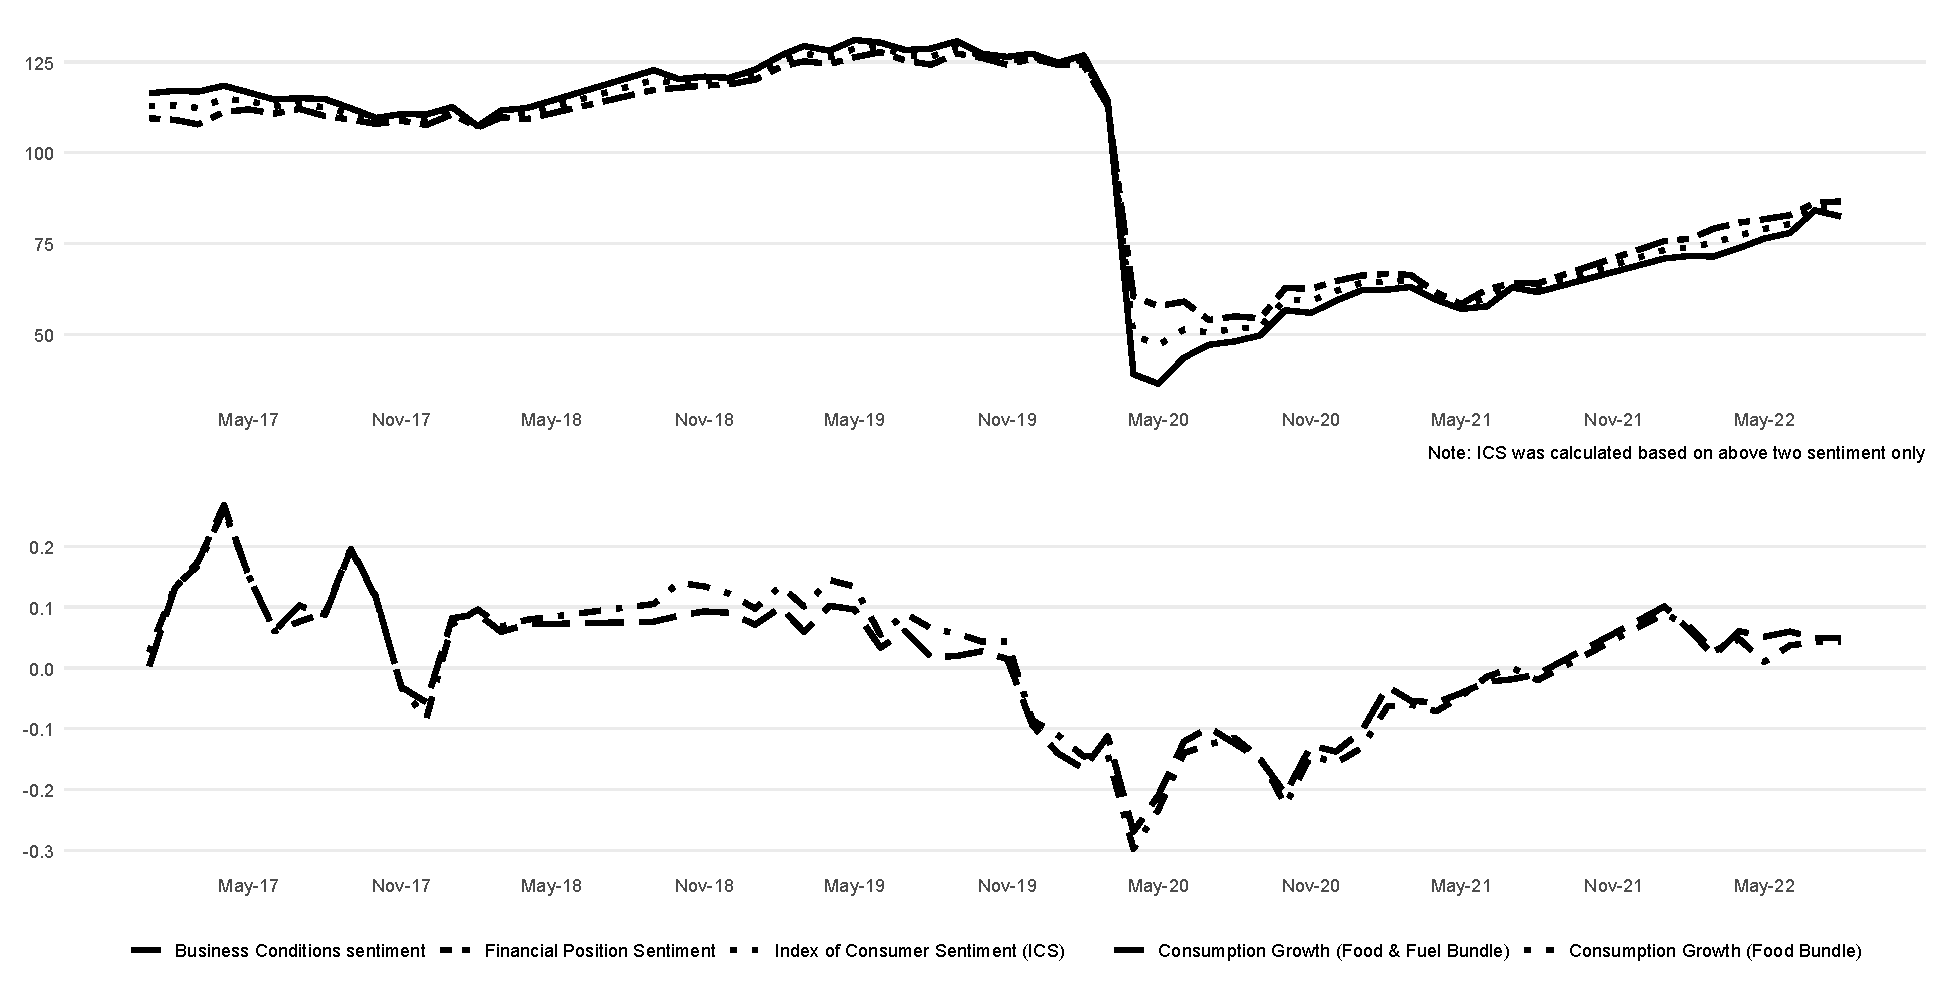
\includegraphics[width=\linewidth,height=1.5\textheight,keepaspectratio]{images/ics_new.pdf}

}

\caption{\label{fig-ics}Index of Consumer Sentiment and Aggregate
Consumption Growth}

\end{figure}%

While the upper panel of the figure above plots the sentiments, the
lower panel depicts the aggregate consumption growth of India from May
2017 to October 2022, calculated on the basis of the food bundle and the
food \& fuel bundle, respectively. Note, the upper and the lower panel
of the figure portrays a significant co-movement between the household
sentiments and their consumption growth. It also shows that, along with
the household sentiments, the Covid-19 pandemic also badly affects their
consumption, from which the Indian households are yet to fully recover.
Observing their co-movement, we calculate the correlation between the
aggregate consumption growth with -- (a) the balance statistics of
question III, (b) the balance statistics of question IV, and (c) the ICS
to assess their interrelationship. We find that the correlation
coefficients are positive and significant at the 1\% level\footnote{See,
  Correlation Matrix(Table~\ref{tbl-correlation}) in the appendix.}.
Note, both the figure above as well as the lower panel of the
correlation matrix table portrays the lasting impact of the Covid-19
pandemic on the psyche and the spending decisions of the Indian
households. To fully uncover their interrelationship, and to examine the
predictive power of sentiments, we use a full-blown regression analysis
based on the Euler equation framework in the next section.

\subsection{The Baseline OLS
Estimation}\label{the-baseline-ols-estimation}

After observing the positive association between consumption growth, and
sentiments, we estimate Equation~\ref{eq-sol1} by OLS using the data of
Indian households from May 2017 to October 2022. Equation~\ref{eq-sol1}
is adopted from Souleles
(\citeproc{ref-souleles_expectations_2004}{2004}).

\begin{equation}\phantomsection\label{eq-sol1}{
\Delta ln\left(c_{h\left(t+1\right)}^j\right){=b_0 time+b_1W_{h\left(t+1\right)}}+b_2Q_{ht}^j+\eta_{h\left(t+1\right)}
}\end{equation}

The dependent variable of Equation~\ref{eq-sol1},
\(\Delta ln\left(c_{h\left(t+1\right)}^j\right)\) is the consumption
growth for the household \(h\), belonging to the \(j^{th}\) geographical
location at period, \((t+1)\). We have calculated consumption growth
either on the basis of the food bundle, or the food \& fuel bundle for
as explained above. Our coefficient of interest is, \(b_2\) -- the
excess sensitivity parameter. A statistically significant excess
sensitivity parameter implies the presence of the excess sensitivity of
consumption to sentiments, and it also represents the violation of the
PIH. Following Ludvigson (\citeproc{ref-Ludvigson2004}{2004}), we use
the futuristic sentiments of the households h, belonging to the
\(j^{th}\) geographical location at time \((t+1)\),
\(\ Q_{h\left(t+1\right)}^j\) as determinants of consumption growth in
Equation~\ref{eq-sol1}. To estimate Equation~\ref{eq-sol1}, we use two
such futuristic measures of household sentiments -- (i) one period ahead
future sentiments for the household's own financial position
\(\left(Q_{FP}\right)\); and (ii) one period ahead sentiments about the
future business condition \(\left(Q_{BC}\right)\).

Along with sentiments, we also include following additional controls in
Equation~\ref{eq-sol1} - (i) time dummy - \(time\) to to control impact
of aggregate shocks on the consumption growth of the households. The
time dummy takes the value 1 for the said time period, and 0 otherwise.
For a panel data with large cross sectional units, and small time
dimension; the inclusion of time dummy helps to achieve consistency when
aggregate shocks are assumed to uniformly affect all households
(\citeproc{ref-chamberlain1984panel}{Chamberlain, 1984}). and (ii) we
also control for the preference shock, determined by the change in
number of kids, change in number of adults, and the age of the household
head in \(W_{h\left(t+1\right)}\) as proxies of the preference shocks
(\citeproc{ref-souleles_expectations_2004}{Souleles, 2004}).\footnote{Section~\ref{sec-3}
  shows that, PIH holds when the homogeneous discount is equal to the
  inverse of the gross interest rate, \(\beta=R^{-1}\). However, the
  discount factor can also vary across households. Alongside the
  preference shock, variables included in \(W_h(t+1)\) in
  Equation~\ref{eq-sol1} captures the cross-sectional heterogeneity of
  the discount factor as well.} Table~\ref{tbl-ols_combined} reports the
results obtained from estimating Equation~\ref{eq-sol1} by OLS.

\begin{table}

\caption{\label{tbl-ols_combined}OLS Estimation for Food and Food \& Fuel}

\centering{

\centering


\begin{threeparttable}
\begin{tabular}{l cc cc}
\toprule
& \multicolumn{2}{c}{Food} & \multicolumn{2}{c}{Food \& Fuel} \\ 
\cmidrule(lr){2-3} \cmidrule(lr){4-5}
 & (1) & (2) & (3) & (4)  \\ 
\midrule
$Q_{FP}$  & 0.009***  &  & 0.054***  &  \\ 
          & (0.002)  &  & (0.002)  &  \\ 
\addlinespace
$Q_{BC}$  &   & 0.003***  &   & 0.003***  \\ 
          &   & (0.002)  &   & (0.002)  \\ 
\addlinespace
Age       & -0.000***  & -0.000***  & -0.000***  & -0.000***  \\ 
          & (0.002)  & (0.000)  & (0.002)  & (0.000)  \\ 
\addlinespace
$\Delta$ kids  & 0.011***  & 0.011***  & 0.07***  & 0.07***  \\ 
              & (0.012)  & (0.012)  & (0.002)  & (0.002)  \\ 
\addlinespace
$\Delta$ adults & 0.038***  & 0.038***  & 0.028***  & 0.002***  \\ 
                & (0.002)  & (0.002)  & (0.002)  & (0.002)  \\ 
\midrule
Time Dummies & Yes & Yes & Yes & Yes  \\ 
Number of Observations & 58,871 & 58,871 & 58,871 & 58,871  \\ 
\bottomrule
\end{tabular}
\end{threeparttable}
\caption*{\footnotesize \textbf{Note:} : (i) Age represents the age of the household head, (ii) $\Delta$ kids, and $\Delta$ adults  represent change in number of kids, and change in number of adults respectively, (iii)***, **, * represent significance at 1\%, 5\%, and 10\% level respectively.}

}

\end{table}%

Table~\ref{tbl-ols_combined} shows that, the coefficients of \(Q_{FP}\)
and \(Q_{BC}\) are positive, and significant at 1\% level.
Table~\ref{tbl-ols_combined} further reveal that, the raw sentiments of
Indian household's about their one period ahead financial position
\(\left(Q_{FP}\right)\), can explain only \(0.9\%\) variation of the
consumption growth of the food bundle, and \(5.4\%\) variation of the
food \& fuel bundle. On the other hand, we find that the raw sentiments
of Indian household's about their one period ahead business condition
\(\left(Q_{BC}\right)\), can explain only \(0.3\%\) variation of the
consumption growth of both the food bundle, and the food \& fuel bundle.
In effect, the results of Table~\ref{tbl-ols_combined} imply that, the
sentiments of Indian households contains additional information, beyond
that is in the current consumption, required to predict the future
consumption, which refutes the prediction of PIH as discussed above.

\subsection{The GMM Estimation}\label{the-gmm-estimation}

Toussaint-Comeau \& McGranahan
(\citeproc{ref-toussaint2006variations}{2006}) argues that sentiment
contains rich demographic-specific information of spending patterns for
US households. Similarly, Blendon et al.
(\citeproc{ref-blendon1997}{1997}) argues that individuals form their
sentiments mostly by processing information obtained during
conversations with their neighbors at the backyard of their house. This
implies that the geographical location of the individuals, along with
their education, income, and other demographic characteristics, plays an
important role in the formation of individual sentiments. As a result,
we re-estimate Equation~\ref{eq-sol1} through GMM by using,
\ensuremath{\mathbf{Z} = [\text{age} \times \text{time},\, \text{income} \times \text{time},\, \text{location},\, \text{marital status},\, \text{gender of household head},\, \text{nature of occupation},\, \text{education},\, \\ \log (\text{real income})]}.
We have used, \(Z\), the instruments of Indian households following
Souleles (\citeproc{ref-souleles_expectations_2004}{2004}), and estimate
Equation~\ref{eq-sol1} by GMM. Table~\ref{tbl-gmm_combined} reports the
results of the GMM estimation. Note, comparison of the coefficients of
sentiments, \(b_2\) obtained from the GMM estimation with that of the
OLS estimation of Equation~\ref{eq-sol1} allows us assessing to what
extent the part of the household sentiments, explained by the chosen
instruments, \(Z\) outperforms the raw sentiments in predicting the
consumption growth of Indian households.

\begin{table}

\caption{\label{tbl-gmm_combined}GMM Estimation for Food and Food \& Fuel}

\centering{

\centering


\begin{threeparttable}
\resizebox{\linewidth}{!}{%
\begin{tabular}{l cc cc}
\toprule
& \multicolumn{2}{c}{Food} & \multicolumn{2}{c}{Food \& Fuel} \\ 
\cmidrule(lr){2-3} \cmidrule(lr){4-5}
 & (1) & (2) & (3) & (4) \\ 
\midrule
$Q_{FP}$  & 0.555*** &  & 0.695*** &  \\ 
          & (0.00)   &  & (0.030)  &  \\ 
\addlinespace
$Q_{BC}$  &   & 0.345***  &   & 0.661***  \\ 
          &   & (0.038)   &   & (0.037)   \\ 
\addlinespace
Age       & -0.001***  & -0.001***  & -0.001***  & -0.001***  \\ 
          & (0.000)    & (0.000)    & (0.000)    & (0.000)    \\ 
\addlinespace
$\Delta$ kids  & 0.009  & -0.007  & 0.010  & -0.015  \\ 
              & (0.37)  & (0.009)  & (0.012)  & (0.012)  \\ 
\addlinespace
$\Delta$ adults & 0.018  & 0.041**  & -0.342  & -0.010  \\ 
                & (0.46)  & (0.021)  & (0.026)  & (0.026)  \\ 
\midrule
Time Dummies & Yes & Yes & Yes & Yes  \\ 
Number of Observations & 56,211 & 56,211 & 56,211 & 56,211  \\ 
\bottomrule
\end{tabular}
}
\end{threeparttable}
\caption*{\footnotesize \textbf{Note:} : (i) Age represents the age of the household head, (ii) $\Delta$ kids, and $\Delta$ adults  represent change in number of kids, and change in number of adults respectively, (iii)***, **, * represent significance at 1\%, 5\%, and 10\% level respectively.}

}

\end{table}%

Table~\ref{tbl-gmm_combined} show that the coefficients of \(Q_{FP}\)
and \(Q_{BC}\) are positive and significant at the 1\% level. Like our
OLS estimation, the GMM estimation also represents the presence of
excess sensitivity of consumption to sentiments and the violation of the
PIH as explained before. Moreover, Table~\ref{tbl-gmm_combined} show
that while \(Q_{FP}\) explains \(55.5\%\) variation of the consumption
growth for the food bundle, it explains almost \(70\%\) variation of the
food \& fuel bundle. Similarly, results of our GMM estimation reported
in Table~\ref{tbl-gmm_combined} also show that while \(Q_{BC}\) explains
\(34.5\%\) variation of the consumption growth for the food bundle, it
explains almost \(66\%\) variation of the food \& fuel bundle. A cursory
comparison of the results of Table~\ref{tbl-gmm_combined} with that of
Table~\ref{tbl-ols_combined} shows that the part of the sentiments of
Indian households, explained by their geographical location, income,
education, and demographics, is a superior predictor of their
consumption growth than the raw sentiments itself. Our results reported
in Table~\ref{tbl-gmm_combined} also show that the fuel consumption of
Indian households is more sensitive to the sentiments than the food
consumption.

\subsection{The Covid-19 Pandemic and the Role of Sentiments as
Predictor of Consumption
Growth}\label{the-covid-19-pandemic-and-the-role-of-sentiments-as-predictor-of-consumption-growth}

Figure~\ref{fig-ics} shows a fantastic co-movement between consumption
growth and the sentiments for the pre-Covid periods. However, it is also
evident from Figure~\ref{fig-ics} that such an exquisite
interrelationship between consumption growth, and sentiment breaks down
in the Covid-periods\footnote{In our analysis, pre-Covid periods is from
  April, 2016 to February, 2020; and the Covid-periods is from March
  2020 to October 2022.}. From Figure~\ref{fig-ics}, and the lower panel
of Table~\ref{tbl-desc} we see that the Covid-19 pandemic has
fundamentally altered the spending pattern of Indian households perhaps
by influencing their income risk through changing the job prospects, and
the health-related risks of the households, reflected in the sluggish
recovery of household sentiments in the Covid-periods\footnote{Figure~\ref{fig-unemp}
  plots the unemployment rate of India. It shows the lasting adverse
  impact of the Covid-19 pandemic on the job prospects of the Indian
  households.}. Although consumption growth recovers faster than
sentiments in the Covid-periods, both sentiment, and consumption growth
remain considerably below their corresponding pre-Covid values as
depicted in Figure~\ref{fig-ics}\footnote{Pistaferri
  (\citeproc{ref-pistaferri2016}{2016}) identifies a similar recovery
  pattern of the US consumption after the global financial crisis. He
  shows that, alongside sentiments, we need to control for debt and net
  worth of the households to explain the dynamics of post-financial
  crisis consumption growth of the US.}.

Therefore, to disentangle the impact of the Covid-19 pandemic on
sentiment, consumption growth, and their interrelationship, we
re-estimate Equation~\ref{eq-sol1} through GMM separately for the
pre-Covid periods, and the Covid-periods. The results for the pre-Covid
periods and Covid-periods are reported in
Table~\ref{tbl-gmm_combined_full}.

\begin{table}

\caption{\label{tbl-gmm_combined_full}GMM Estimation for Food and Food \& Fuel Bundles - Pre-Covid and Covid Periods}

\centering{

\centering


\begin{threeparttable}
\resizebox{\linewidth}{!}{%
\begin{tabular}{l cc cc  cc cc}
\toprule
 & \multicolumn{4}{c}{\textbf{Pre-Covid Period (2016 April - 2020 February)}} & \multicolumn{4}{c}{\textbf{Covid Period (2020 March - 2022 October)}} \\ 
\cmidrule(lr){2-5} \cmidrule(lr){6-9}
 & \multicolumn{2}{c}{\textbf{Food}} & \multicolumn{2}{c}{\textbf{Food \& Fuel}} & \multicolumn{2}{c}{\textbf{Food}} & \multicolumn{2}{c}{\textbf{Food \& Fuel}} \\ 
\cmidrule(lr){2-3} \cmidrule(lr){4-5} \cmidrule(lr){6-7} \cmidrule(lr){8-9}
 & (1) & (2) & (3) & (4) & (5) & (6) & (7) & (8) \\ 
\midrule
$Q_{FP}$  & 0.22***  &         & 0.766***  &         & 0.34***  &         & 0.43***  &         \\ 
          & (0.01)   &         & (0.030)   &         & (0.05)   &         & (0.030)   &         \\ 
\addlinespace
$Q_{BC}$  &          & 0.20*** &          & 0.749*** &          & 0.03  &          & 0.36*** \\ 
          &          & (0.01)  &          & (0.038)  &          & (0.05)  &          & (0.04)  \\ 
\addlinespace
Age       & -0.001*** & -0.001*** & -0.001*** & -0.001*** & -0.002*** & -0.001*** & -0.002*** & -0.001*** \\ 
          & (0.000)   & (0.000)   & (0.000)   & (0.000)   & (0.000)   & (0.000)   & (0.000)   & (0.000)   \\ 
\addlinespace
$\Delta$ Kids  & 0.03  & -0.01  & 0.02  & -0.015  & 0.00  & -0.04  & 0.01  & -0.04  \\ 
               & (0.08) & (0.01) & (0.01) & (0.012) & (0.01) & (0.01) & (0.01) & (0.01) \\ 
\addlinespace
$\Delta$ Adults  & -0.02  & 0.03  & -0.07  & 0.03  & -0.01  & 0.00  & -0.01  & 0.00  \\ 
                 & (0.02) & (0.03) & (0.03) & (0.03) & (0.03) & (0.03) & (0.03) & (0.03) \\ 
\midrule
Time Dummies  & Yes  & Yes  & Yes  & Yes  & Yes  & Yes  & Yes  & Yes  \\ 
Observations  & 38,131  & 38,131  & 38,131  & 38,131  & 17,400  & 17,400  & 17,400  & 17,400  \\ 
\bottomrule
\end{tabular}
}
\end{threeparttable}
\caption*{\footnotesize \textbf{Note:} : (i) Age represents the age of the household head, (ii) $\Delta$ kids, and $\Delta$ adults  represent change in number of kids, and change in number of adults respectively, (iii)***, **, * represent significance at 1\%, 5\%, and 10\% level respectively.}

}

\end{table}%

To explain the reduced predictive capacity of sentiments note that,
Covid-19 pandemic has a lasting impact on the job prospects, health
conditions, and the psyche of the households as noted before. The
enduring adverse impact of the Covid-19 pandemic becomes more severe for
a developing country like India where, households do not enjoy the
widespread and permanent safety nets of the social security schemes like
the developed countries. In effect, the Covid-19 pandemic significantly
changes income risk of the Indian households, which in turn considerably
alters the pattern as well as the determinants of their spending
decisions in the Covid-periods. The changing pattern and the
determinants of the household spending decisions, and correspondingly
the precautionary savings motive significantly reduces the predictive
capacity of household sentiments in the Covid-periods.

\subsection{Consistency and the Spurious Excess Sensitivity - The Role
of Forecast
Error}\label{consistency-and-the-spurious-excess-sensitivity---the-role-of-forecast-error}

Jappelli \& Pistaferri (\citeproc{ref-jappelli2017economics}{2017}) and
Christelis et al. (\citeproc{ref-Christelis2016}{2020}) argue about
endogeneity arising from the correlation between the forecast errors of
consumption growth in the Euler equation-based estimation. To achieve
consistency by addressing such endogeneity, they suggest using survey
data-based estimates of expected consumption growth and expected
consumption risk for the estimation. On the other hand, to address the
spurious excess sensitivity of consumption to sentiments, Souleles
(\citeproc{ref-souleles_expectations_2004}{2004}) calculates the
forecast error of household sentiments from the survey data and uses it
as one of the covariates in his estimation. Following Souleles
(\citeproc{ref-souleles_expectations_2004}{2004}), we also calculate the
forecast errors for Indian households for their own financial position
and use it as one of the covariates in our estimation to address the
spurious excess sensitivity of consumption to sentiments and to achieve
consistency as well. We calculate the forecast errors by taking the
difference of question II and question III mentioned in
Section~\ref{sec-2}. As a result, the forecast error, \(FE_{FP}\), takes
discrete values between -2 to +2 in our analysis. Using this measure of
forecast errors, we estimate Equation~\ref{eq-sol2} through OLS and also
through GMM. Results of the OLS estimation and GMM estimation of
Equation~\ref{eq-sol2} for the food bundle and for the food \& fuel
bundle are reported below:

\begin{equation}\phantomsection\label{eq-sol2}{
\Delta ln\left(c_{h\left(t+1\right)}^j\right){=b_0time+b_1W_{h\left(t+1\right)}}+b_2Q_{ht}^j+b_3{FE}_{PC,ht}+\omega_{h\left(t+1\right)}
}\end{equation}

\FloatBarrier

\begin{table}

\caption{\label{tbl-fe_ols_gmm}Estimation for Food Bundle and Food \& Fuel Bundle after Controlling for Forecast Error}

\centering{

\centering


\begin{threeparttable}
\begin{tabular}{lcccc}
\toprule
 & \multicolumn{2}{c}{OLS} & \multicolumn{2}{c}{GMM} \\
\cmidrule(lr){2-3} \cmidrule(lr){4-5}
 & Food & Food \& Fuel & Food & Food \& Fuel \\
\midrule
$Q_{FP}$       & 0.03***  & 0.023***  & 0.476***  & 0.461***  \\
               & (0.003)  & (0.003)   & (0.00)    & (0.00)    \\
$FE_{FP}$      & 0.027*** & 0.023***  & 0.53***   & 0.497***  \\
               & (0.002)  & (0.002)   & (0.00)    & (0.00)    \\
Age            & -0.000*** & -0.000*** & -0.001    & -0.000    \\
               & (0.000)   & (0.000)   & (0.96)    & (0.92)    \\
$\Delta$ kids  & 0.011*** & 0.06***   & 0.017     & 0.003     \\
               & (0.012)  & (0.003)   & (0.012)   & (0.02)    \\
$\Delta$ adults& 0.039*** & 0.029***  & 0.009     & 0.011     \\
               & (0.002)  & (0.002)   & (0.71)    & (0.62)    \\
\midrule
Time Dummies   & Yes      & Yes       & Yes       & Yes       \\
Observations   & 53,312   & 53,312    & 53,312    & 53,312    \\
\bottomrule
\end{tabular}
\end{threeparttable}
\caption*{\footnotesize \textbf{Note:} : (i) Age represents the age of the household head, (ii) $\Delta$ kids, and $\Delta$ adults  represent change in number of kids, and change in number of adults respectively, (iii) FE represents forecast errors of the financial position, (iv) ***, **, * represent significance at 1\%, 5\%, and 10\% level respectively.}

}

\end{table}%

\begin{table}

\caption{\label{tbl-gmm_fe}GMM Estimation for Food and Food \& Fuel Bundles - Pre-Covid and Covid Periods after controlling for forecast errors}

\centering{

\centering



\begin{threeparttable}
\resizebox{\linewidth}{!}{%
\begin{tabular}{l cc cc}
\toprule
 & \multicolumn{2}{c}{\textbf{Pre-Covid (2016 April - 2020 February)}} & \multicolumn{2}{c}{\textbf{Covid (2020 March - 2022 October)}} \\ 
\cmidrule(lr){2-3} \cmidrule(lr){4-5}
 & Food  & Food \& Fuel  & Food  & Food \& Fuel  \\ 
\midrule
$Q_{FP}$  & 0.25***  & 0.717***  & 0.31***  & 0.20***  \\ 
          & (0.002)  & (0.030)   & (0.06)   & (0.06)   \\ 
\addlinespace
$FE_{FP}$ & 0.613*** & 0.613***  & 0.42***  & 0.68***  \\ 
          & (0.061)  & (0.061)   & (0.009)  & (0.061)  \\ 
\addlinespace
Age       & -0.001*** & -0.001*** & -0.001*** & -0.001*** \\ 
          & (0.000)   & (0.000)   & (0.000)   & (0.000)   \\ 
\addlinespace
$\Delta$ Kids  & 0.017  & 0.017  & -0.03  & -0.03  \\ 
               & (0.012) & (0.012) & (0.02) & (0.02) \\ 
\addlinespace
$\Delta$ Adults  & -0.009  & -0.009**  & -0.01  & -0.01**  \\ 
                 & (0.71)  & (0.71)    & (0.06) & (0.06)  \\ 
\midrule
Time Dummies  & Yes  & Yes  & Yes  & Yes  \\ 
Observations  & 37,717  & 37,717  & 12,615  & 12,615  \\ 
\bottomrule
\end{tabular}
}
\end{threeparttable}
\caption*{\footnotesize \textbf{Note:} : (i) Age represents the age of the household head, (ii) $\Delta$ kids, and $\Delta$ adults  represent change in number of kids, and change in number of adults respectively, (iii) FE represents forecast errors of the financial position, (iv) ***, **, * represent significance at 1\%, 5\%, and 10\% level respectively.
}

}

\end{table}%

Results reported in {Table~\ref{tbl-fe_ols_gmm} and
Table~\ref{tbl-gmm_fe}} validate the robustness of our previous results.
It shows that household sentiments have significant predicting power and
influence business cycles, and it should be properly controlled to
forecast consumption. The results of OLS and GMM estimation of
Equation~\ref{eq-sol2} separately for the pre-Covid periods and
Covid-periods, reported in {Table~\ref{tbl-fe_ols_gmm} and
Table~\ref{tbl-gmm_fe}} are characteristically identical with the
results reported in Table~\ref{tbl-gmm_combined}, re-establishing the
robustness of our results.

\section{Conclusion}\label{sec-5}

Identifying the determinants of sentiment, and examining its role in
forecasting spending has long intrigued econometricians and policy
makers. While early research relied primarily on national or state-level
aggregate data to examine this relationship, the field has evolved
methodologically with the increasing adoption of microeconomic survey
data. This methodological shift offers enhanced analytical power for
assessing the predictive capacity of sentiment indicators on consumption
dynamics. Our paper represents the first comprehensive attempt to
examine the predictive power of sentiment on consumption growth and to
test the implications of the rational expectation based Permanent
Income/Life Cycle Hypothesis using household-level data from India.

To examine whether sentiment can forecast household consumption growth
in India, we employ the comprehensive longitudinal microdata from the
Consumer Pyramid Household Survey (CPHS). Our novel methodological
approach involves constructing two distinct expenditure-minimizing
consumption bundles: (i) food bundle, and (ii) food \& fuel bundle.
These bundles serve as household-specific real consumption expenditure
measures, effectively preserving the rich cross-sectional heterogeneity
of the Indian economy. We utilize two forward-looking sentiment
indicators: households' expectations regarding their future financial
position and their perceptions of future business conditions. By using
these sentiment measures within an Euler equation framework, we
simultaneously test whether household sentiment indicators possess
significant predictive power for consumption growth and whether
consumption exhibits excess sensitivity to sentiment
fluctuations---findings that would test the validity of the Permanent
Income Hypothesis (PIH) in the Indian household context.

We show that household sentiments explained by geographical location,
income level, educational attainment, and demographic characteristics
are superior predictors of consumption growth compared to raw sentiment
itself. Our results endorse Blendon et al.
(\citeproc{ref-blendon1997}{1997}), who argue that an individual's
neighborhood is instrumental in forming and shaping their sentiments. We
also demonstrate that the fuel consumption of Indian households exhibits
greater sensitivity to sentiments than food consumption. We argue that,
consistent with pre-pandemic patterns, sentiments should remain crucial
for business cycle forecasting in post-pandemic periods, despite
COVID-19 fundamentally altering spending patterns and their underlying
determinants for Indian households by exerting persistent impact on the
psyche of consumers. Our results broadly parallel evidence from
developed economies, contributing to the broader literature on
sentiment-driven consumption and business cycle dynamics.

Finally, to outline our future research agenda, we note that the
sluggish recovery pattern of consumption for Indian households depicted
in Figure~\ref{fig-ics} closely mimics the dynamics of US consumption
growth in the post-Great Recession period. Pistaferri
(\citeproc{ref-pistaferri2016}{2016}) demonstrates that alongside
sentiments, household debt and net worth should be controlled for when
explaining post-Great Recession consumption growth dynamics in the US.
Depending on the availability of data, we plan to explore models that
incorporate health-related risks faced by Indian households due to the
COVID-19 pandemic, alongside their sentiments, liabilities, and net
worth to explain the COVID-period dynamics of consumption growth for
India.

\section*{References}\label{references}
\addcontentsline{toc}{section}{References}

\phantomsection\label{refs}
\begin{CSLReferences}{1}{0}
\bibitem[\citeproctext]{ref-acemoglou1994}
Acemoglu, D., \& Scott, A. (1994). Consumer confidence and rational
expectations: Are agents' beliefs consistent with the theory? \emph{The
Economic Journal}, \emph{104}(422), 1--19.
\url{http://www.jstor.org/stable/2234671}

\bibitem[\citeproctext]{ref-angrist_effect_1992}
Angrist, J. D., \& Krueger, A. B. (1992). The {Effect} of {Age} at
{School} {Entry} on {Educational} {Attainment}: {An} {Application} of
{Instrumental} {Variables} with {Moments} from {Two} {Samples}.
\emph{Journal of the American Statistical Association}, \emph{87}(418),
328--336. \url{https://doi.org/10.1080/01621459.1992.10475212}

\bibitem[\citeproctext]{ref-blendon1997}
Blendon, R. J., Benson, J. M., Brodie, M., Morin, R., Altman, D. E.,
Gitterman, D., Brossard, M., \& James, M. (1997). Bridging the gap
between the public's and economists' views of the economy. \emph{Journal
of Economic Perspectives}, \emph{11}(3), 105--118.
\url{https://doi.org/10.1257/jep.11.3.105}

\bibitem[\citeproctext]{ref-carroll_does_1994}
Carroll, C. D., Fuhrer, J. C., \& Wilcox, D. W. (1994). Does {Consumer}
{Sentiment} {Forecast} {Household} {Spending}? {If} {So}, {Why}?
\emph{The American Economic Review}, \emph{84}(5), 1397--1408.
\url{http://www.jstor.org/stable/2117779}

\bibitem[\citeproctext]{ref-chamberlain1984panel}
Chamberlain, G. (1984). \emph{Panel data', in (z. Griliches and m.
Intriligator, eds.) handbook of econometrics}. North Holland, Amsterdam.

\bibitem[\citeproctext]{ref-Christelis2016}
Christelis, D., Georgarakos, D., Jappelli, T., \& Rooij, M. van. (2020).
Consumption uncertainty and precautionary saving. \emph{The Review of
Economics and Statistics}, \emph{102}(1), 148--161.
\url{https://doi.org/10.1162/rest_a_00819}

\bibitem[\citeproctext]{ref-dominitz2004should}
Dominitz, J., \& Manski, C. F. (2004). How should we measure consumer
confidence? \emph{Journal of Economic Perspectives}, \emph{18}(2),
51--66.

\bibitem[\citeproctext]{ref-hall1978}
Hall, R. E. (1978). Stochastic implications of the life cycle-permanent
income hypothesis: Theory and evidence. \emph{Journal of Political
Economy}, \emph{86}(6), 971--987.
\url{http://www.jstor.org/stable/1840393}

\bibitem[\citeproctext]{ref-immordino2024consumption}
Immordino, G., Jappelli, T., \& Oliviero, T. (2024). Consumption and
income expectations during covid-19. \emph{Review of Economics of the
Household}, \emph{22}(1), 95--116.

\bibitem[\citeproctext]{ref-jappelli2017economics}
Jappelli, T., \& Pistaferri, L. (2017). \emph{The economics of
consumption: Theory and evidence}. Oxford University Press.

\bibitem[\citeproctext]{ref-lahiri_forecasting_2016}
Lahiri, K., Monokroussos, G., \& Zhao, Y. (2016). Forecasting
{Consumption}: The {Role} of {Consumer} {Confidence} in {Real} {Time}
with many {Predictors}. \emph{Journal of Applied Econometrics},
\emph{31}(7), 1254--1275. \url{https://doi.org/10.1002/jae.2494}

\bibitem[\citeproctext]{ref-lahiri_determinants_2016}
Lahiri, K., \& Zhao, Y. (2016). Determinants of {Consumer} {Sentiment}
{Over} {Business} {Cycles}: {Evidence} from the {US} {Surveys} of
{Consumers}. \emph{Journal of Business Cycle Research}, \emph{12}(2),
187--215. \url{https://doi.org/10.1007/s41549-016-0010-5}

\bibitem[\citeproctext]{ref-Ludvigson2004}
Ludvigson, S. C. (2004). Consumer confidence and consumer spending.
\emph{Journal of Economic Perspectives}, \emph{18}(2), 29--50.
\url{https://doi.org/10.1257/0895330041371222}

\bibitem[\citeproctext]{ref-nachane2019plutocratic}
Nachane, D. M., \& Chaubal, A. (2019). The plutocratic bias in the
indian consumer price index. \emph{International Labour Review},
\emph{158}(2), 365--391.

\bibitem[\citeproctext]{ref-pistaferri2016}
Pistaferri, L. (2016). Why has consumption remained moderate after the
great recession. \emph{Boston Fed Conference Proceeding}.

\bibitem[\citeproctext]{ref-priya_sharma2024}
Priya, P., \& Sharma, C. (2024). On transmission channels of energy
prices and monetary policy shocks to household consumption: Evidence
from india. \emph{Energy Economics}, \emph{136}, 107723.
https://doi.org/\url{https://doi.org/10.1016/j.eneco.2024.107723}

\bibitem[\citeproctext]{ref-souleles_expectations_2004}
Souleles, N. S. (2004). Expectations, {Heterogeneous} {Forecast}
{Errors}, and {Consumption}: {Micro} {Evidence} from the {Michigan}
{Consumer} {Sentiment} {Surveys}. \emph{Journal of Money, Credit, and
Banking}, \emph{36}(1), 39--72.
\url{https://doi.org/10.1353/mcb.2004.0007}

\bibitem[\citeproctext]{ref-toussaint2006variations}
Toussaint-Comeau, M., \& McGranahan, L. (2006). Variations in consumer
sentiment across demographic groups. \emph{Economic Perspectives}.

\bibitem[\citeproctext]{ref-vuchelen2004consumer}
Vuchelen, J. (2004). Consumer sentiment and macroeconomic forecasts.
\emph{Journal of Economic Psychology}, \emph{25}(4), 493--506.

\end{CSLReferences}

\newpage

\section*{Appendix}\label{appendix}
\addcontentsline{toc}{section}{Appendix}

\begin{figure}

\centering{

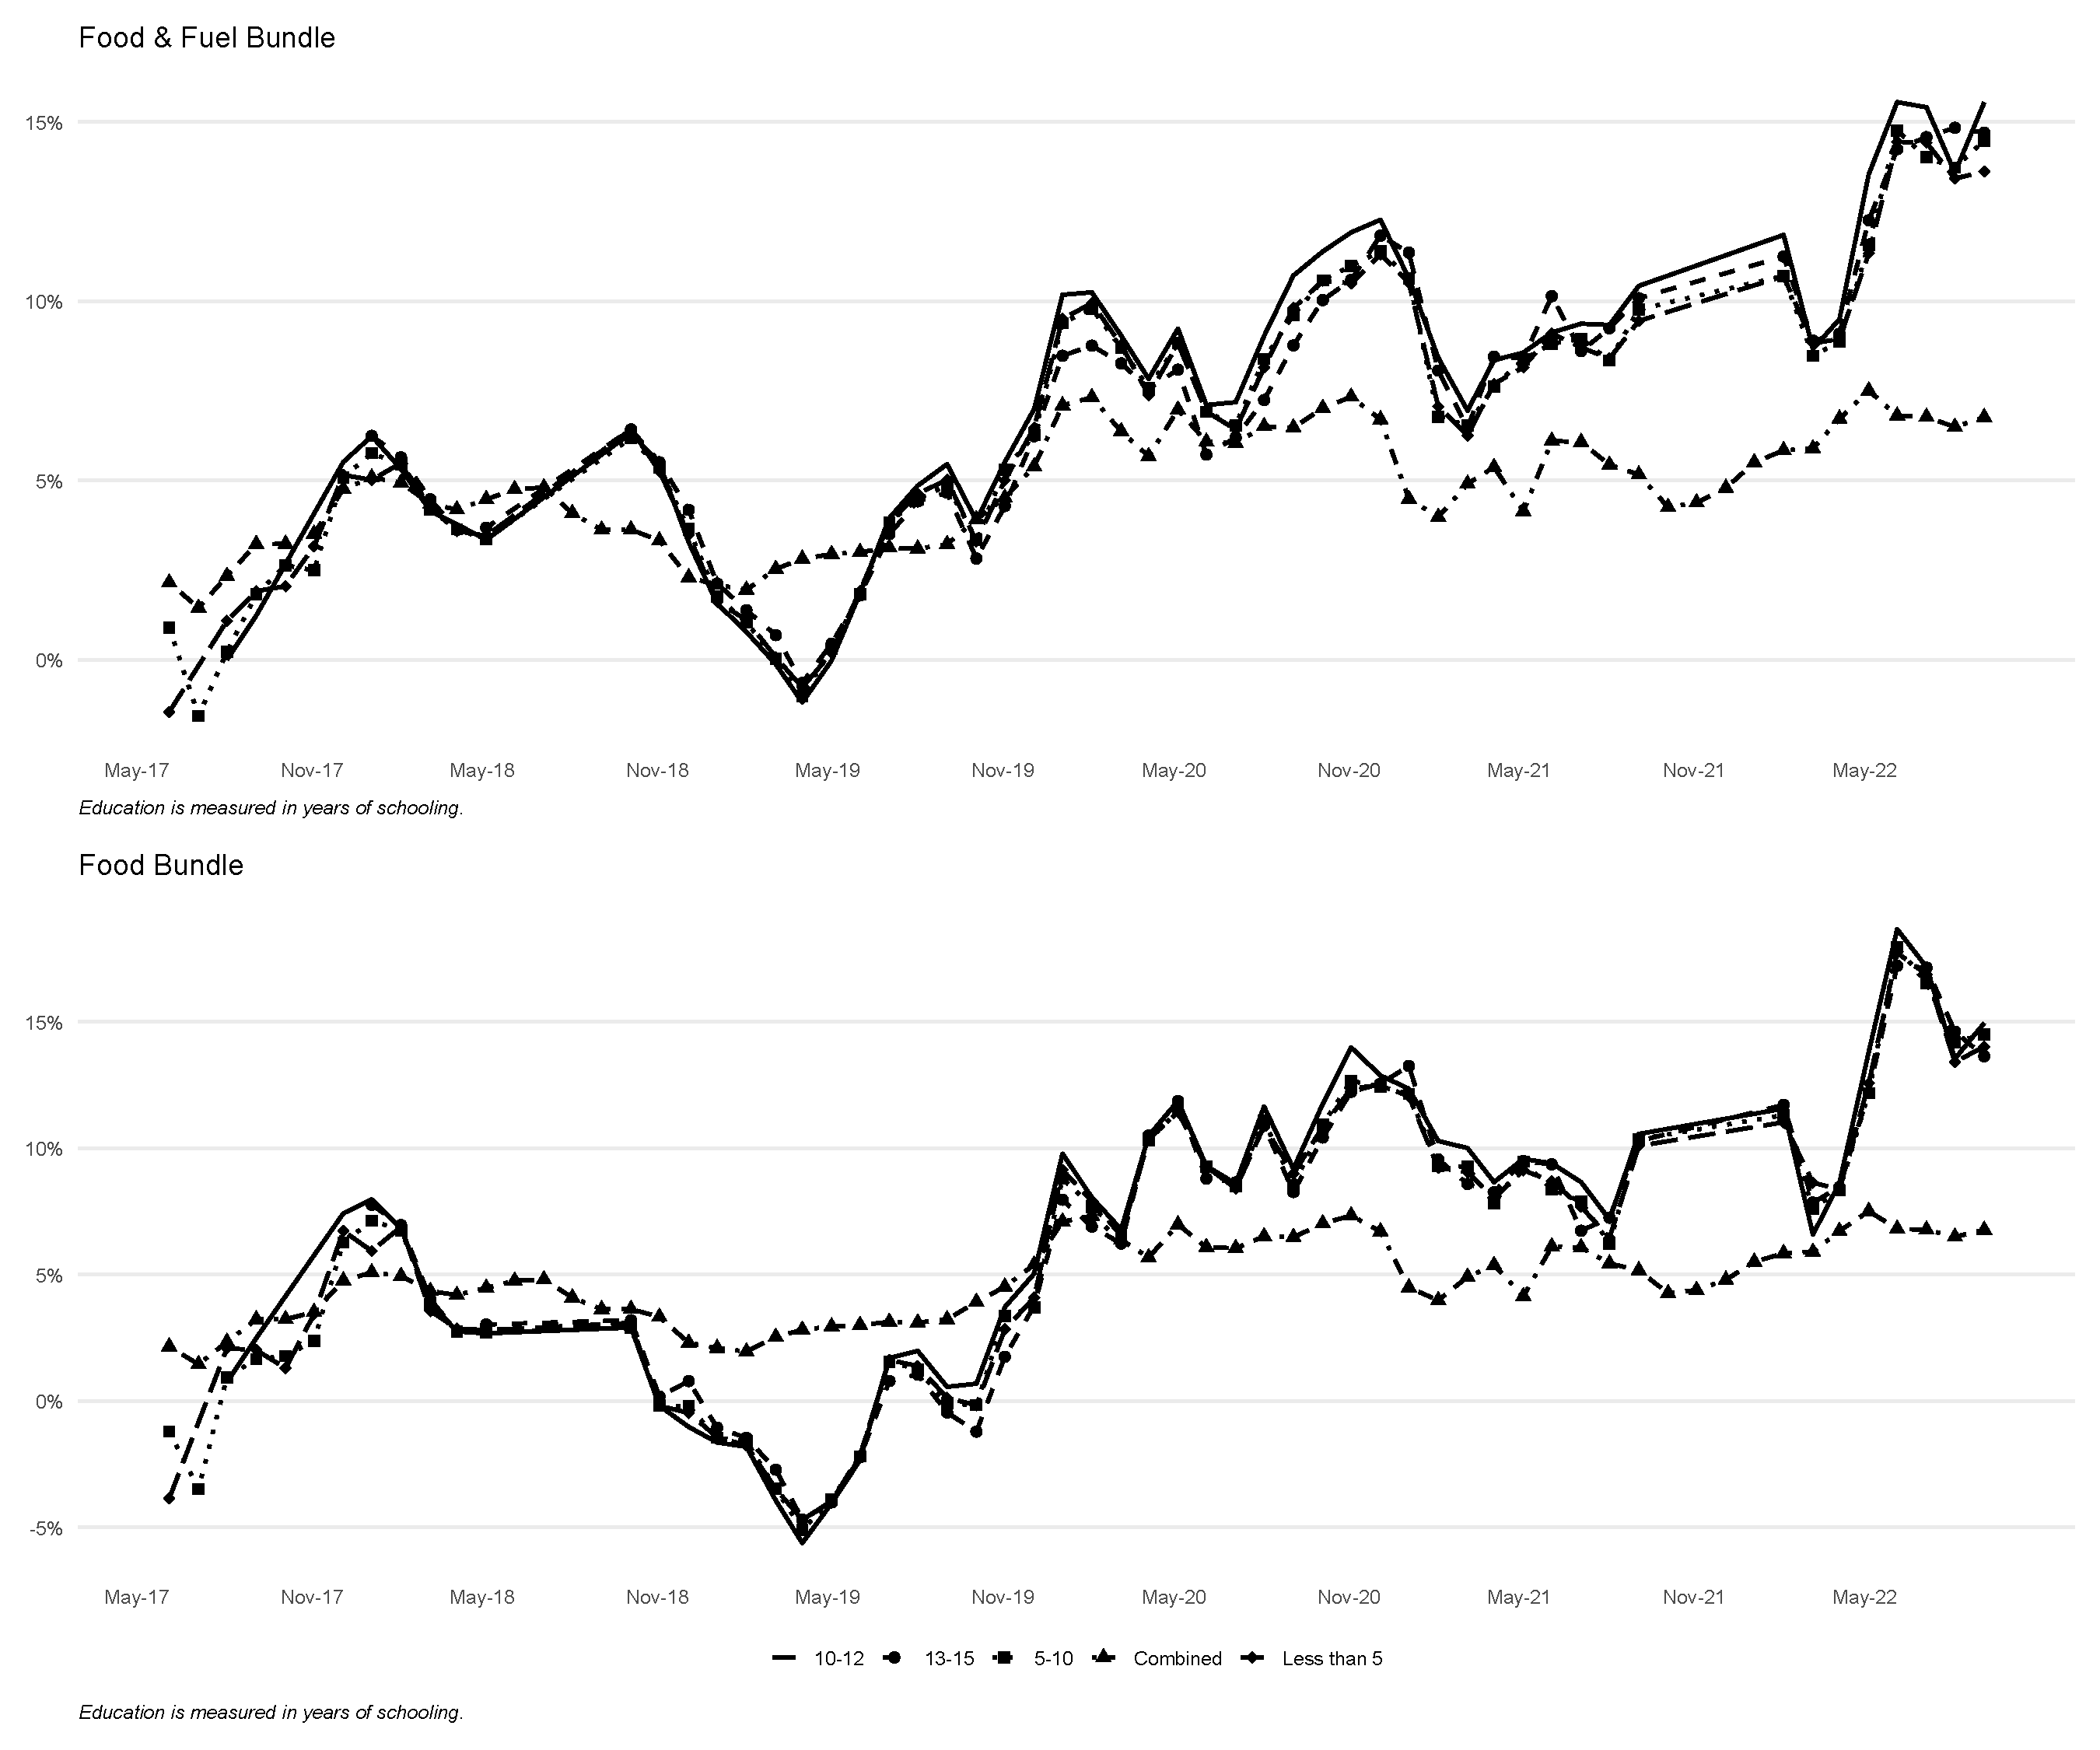
\includegraphics[width=\linewidth,height=1.5\textheight,keepaspectratio]{images/mean_educ_Phmt.pdf}

}

\caption{\label{fig-mean_educ}Cross-sectional Heterogeneity of Average
Aggregate Inflation Rate, and Household Specific Inflation Rate -
Households Classified in terms of Educational Attainment of Household
Head}

\end{figure}%

\begin{figure}

\centering{

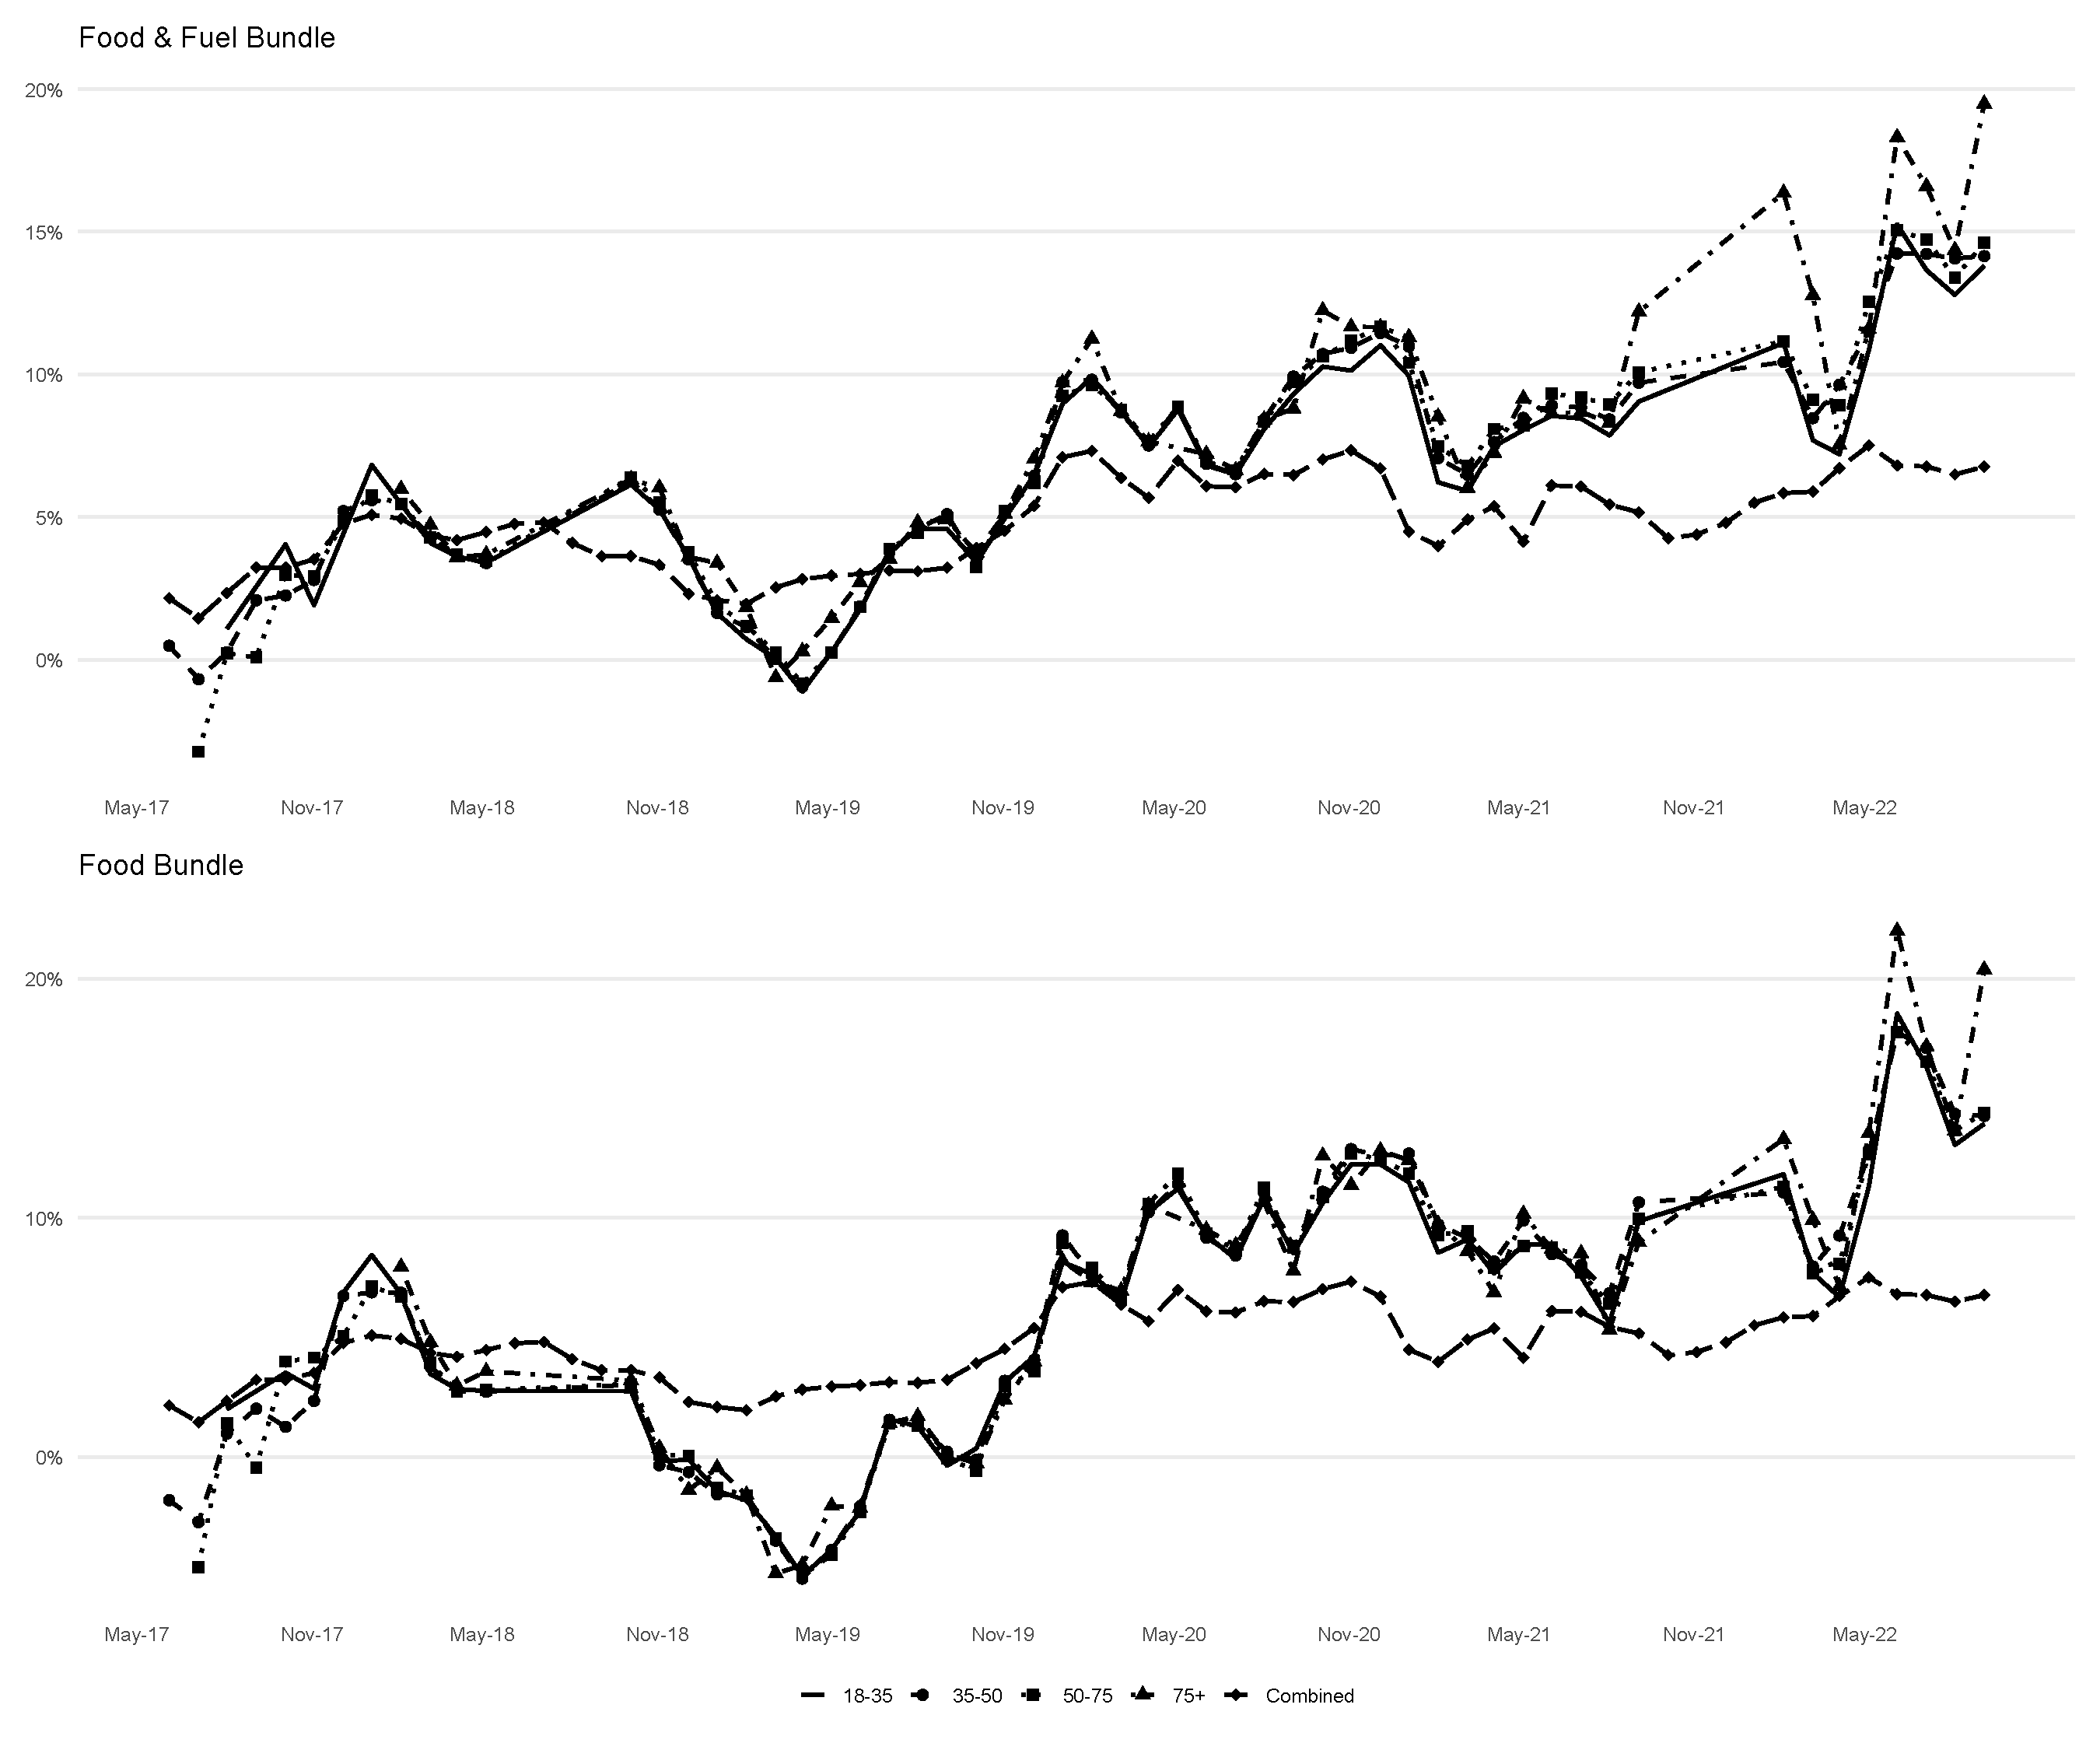
\includegraphics[width=\linewidth,height=1.5\textheight,keepaspectratio]{images/mean_age_cat_Phmt.pdf}

}

\caption{\label{fig-mean_age}Cross-sectional Heterogeneity of Average
Aggregate Inflation Rate, and Household Specific Inflation Rate -
Households Classified in terms of Age of Household Head}

\end{figure}%

\begin{figure}

\centering{

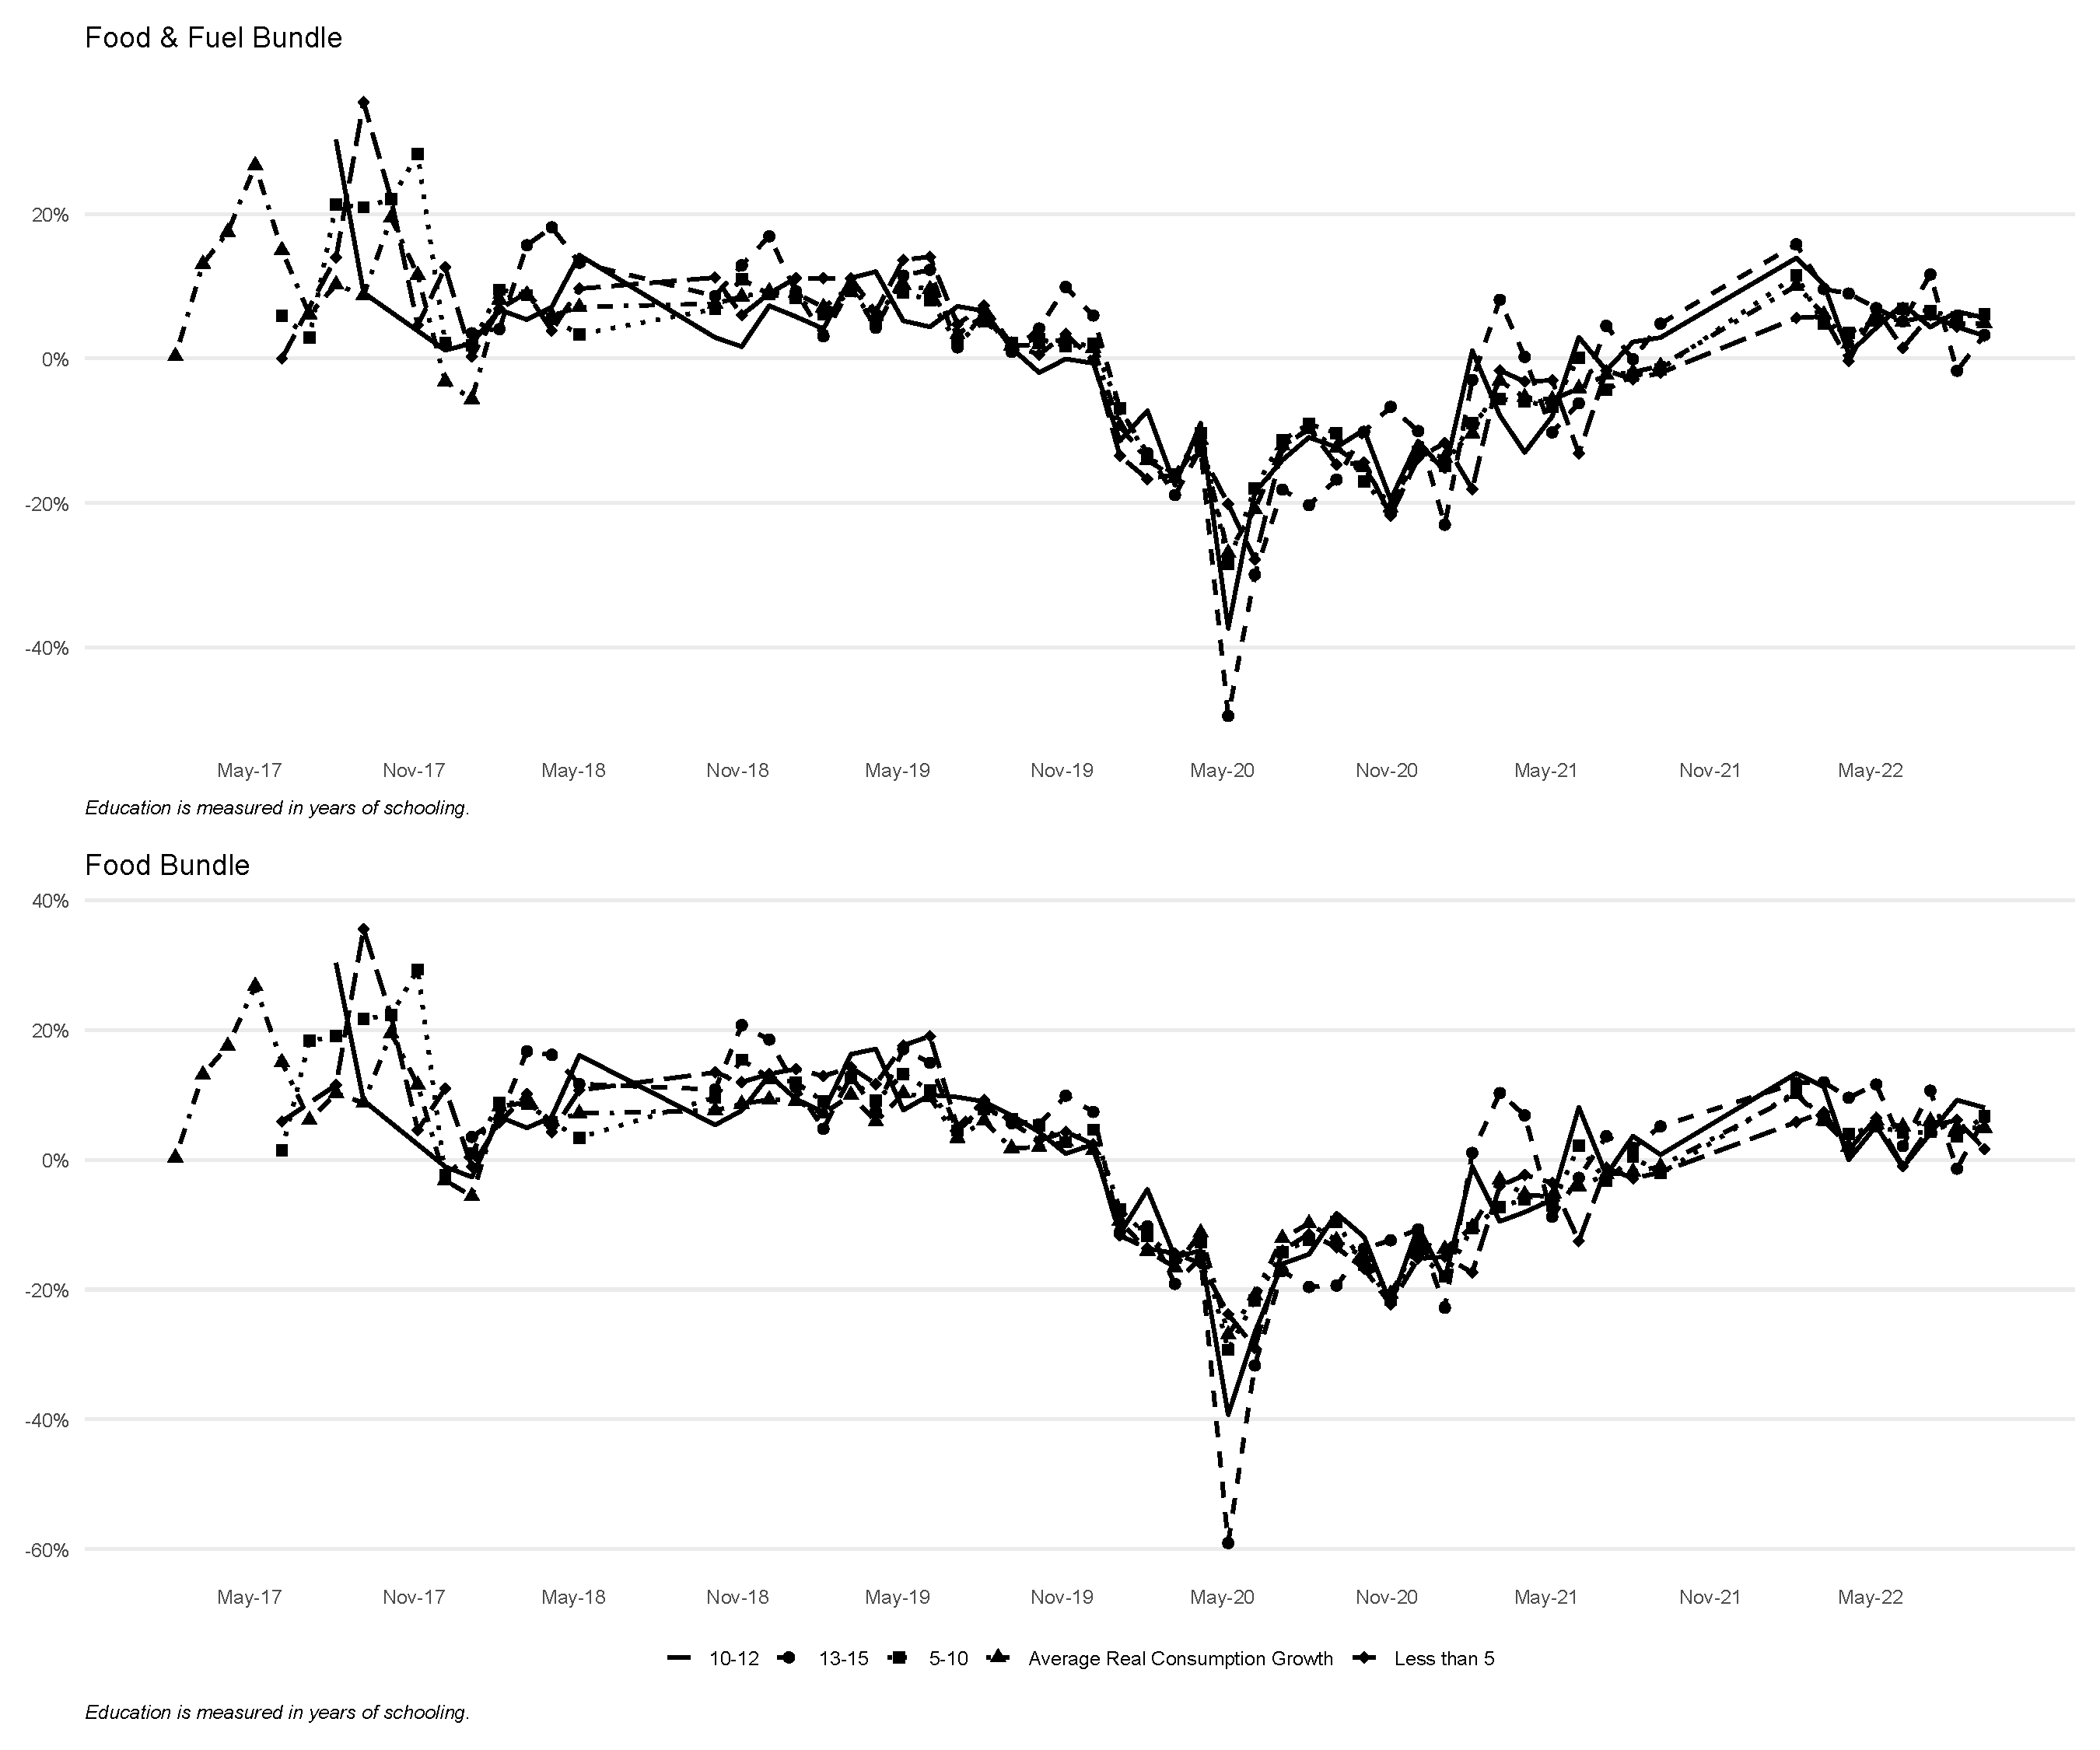
\includegraphics[width=\linewidth,height=1.5\textheight,keepaspectratio]{images/mean_educ_Chmt.pdf}

}

\caption{\label{fig-mean_educ_chmt}Cross-sectional Heterogeneity of
Household Specific Consumption Growth - Households Classified in terms
of Educational Attainment of Household Head}

\end{figure}%

\begin{figure}

\centering{

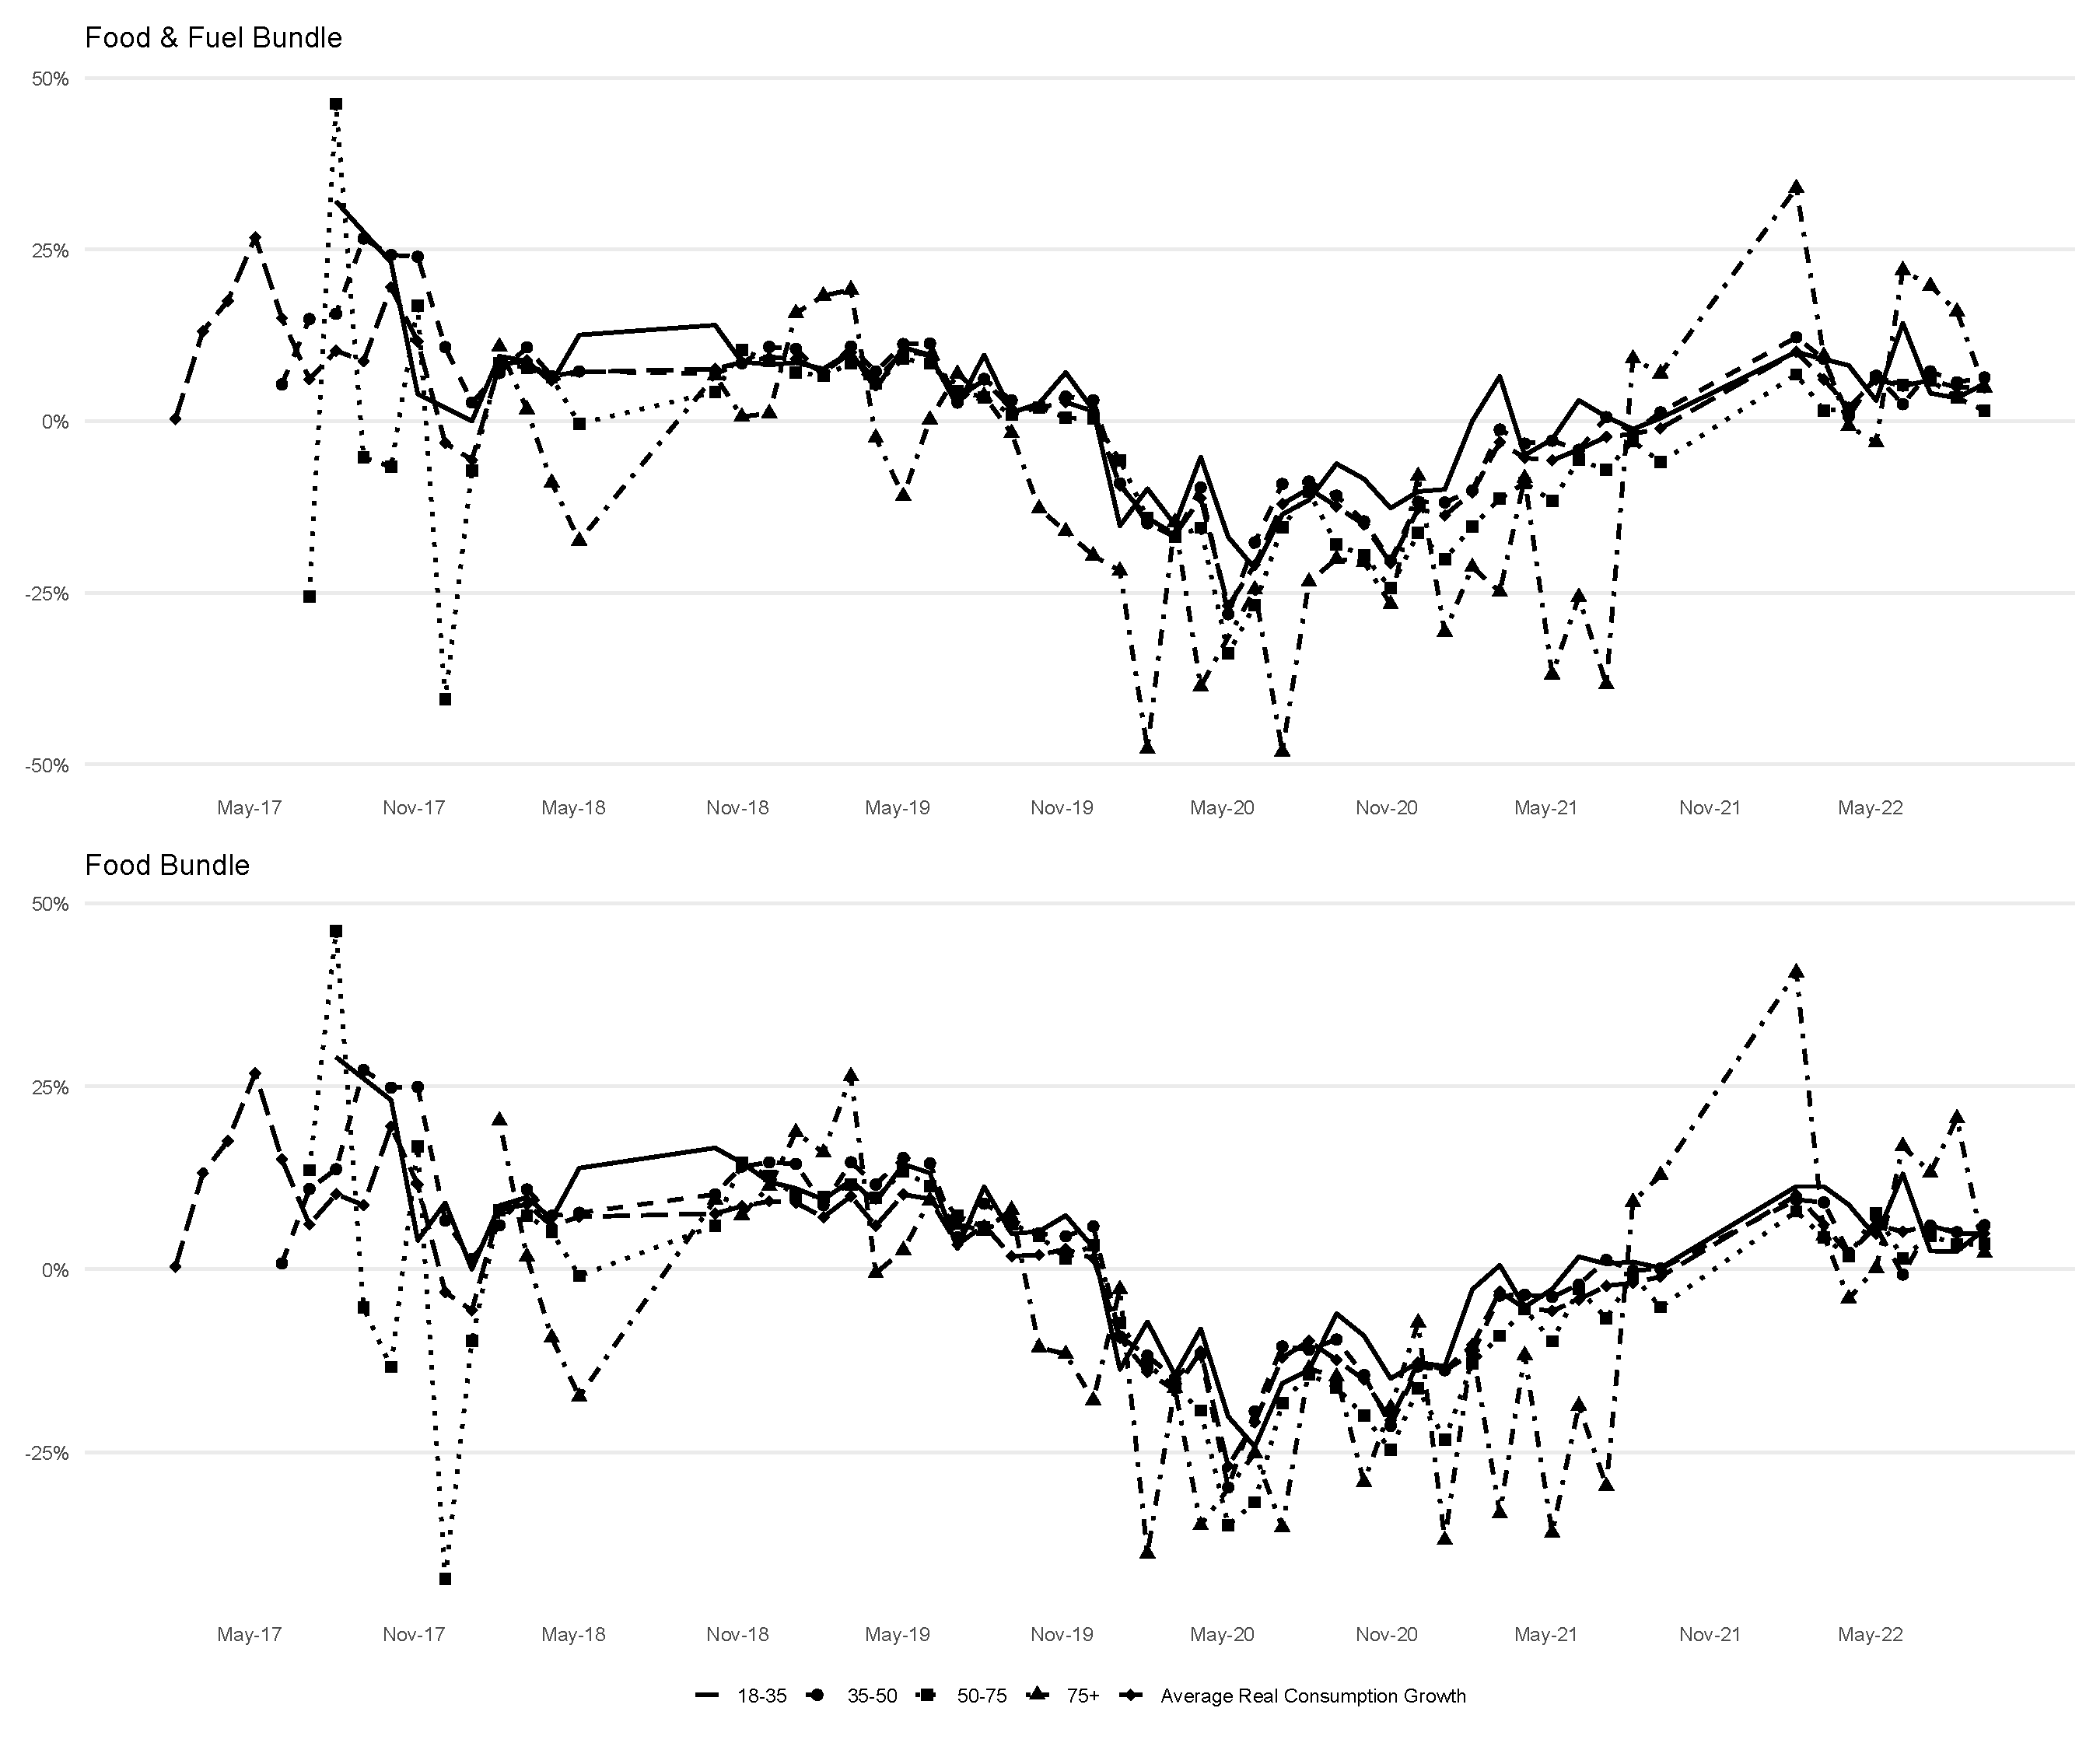
\includegraphics[width=\linewidth,height=1.5\textheight,keepaspectratio]{images/mean_age_cat_Chmt.pdf}

}

\caption{\label{fig-mean_age_chmt}Cross-sectional Heterogeneity of
Household Specific Consumption Growth - Households Classified in terms
of Age of Household Head}

\end{figure}%

\begin{figure}

\centering{

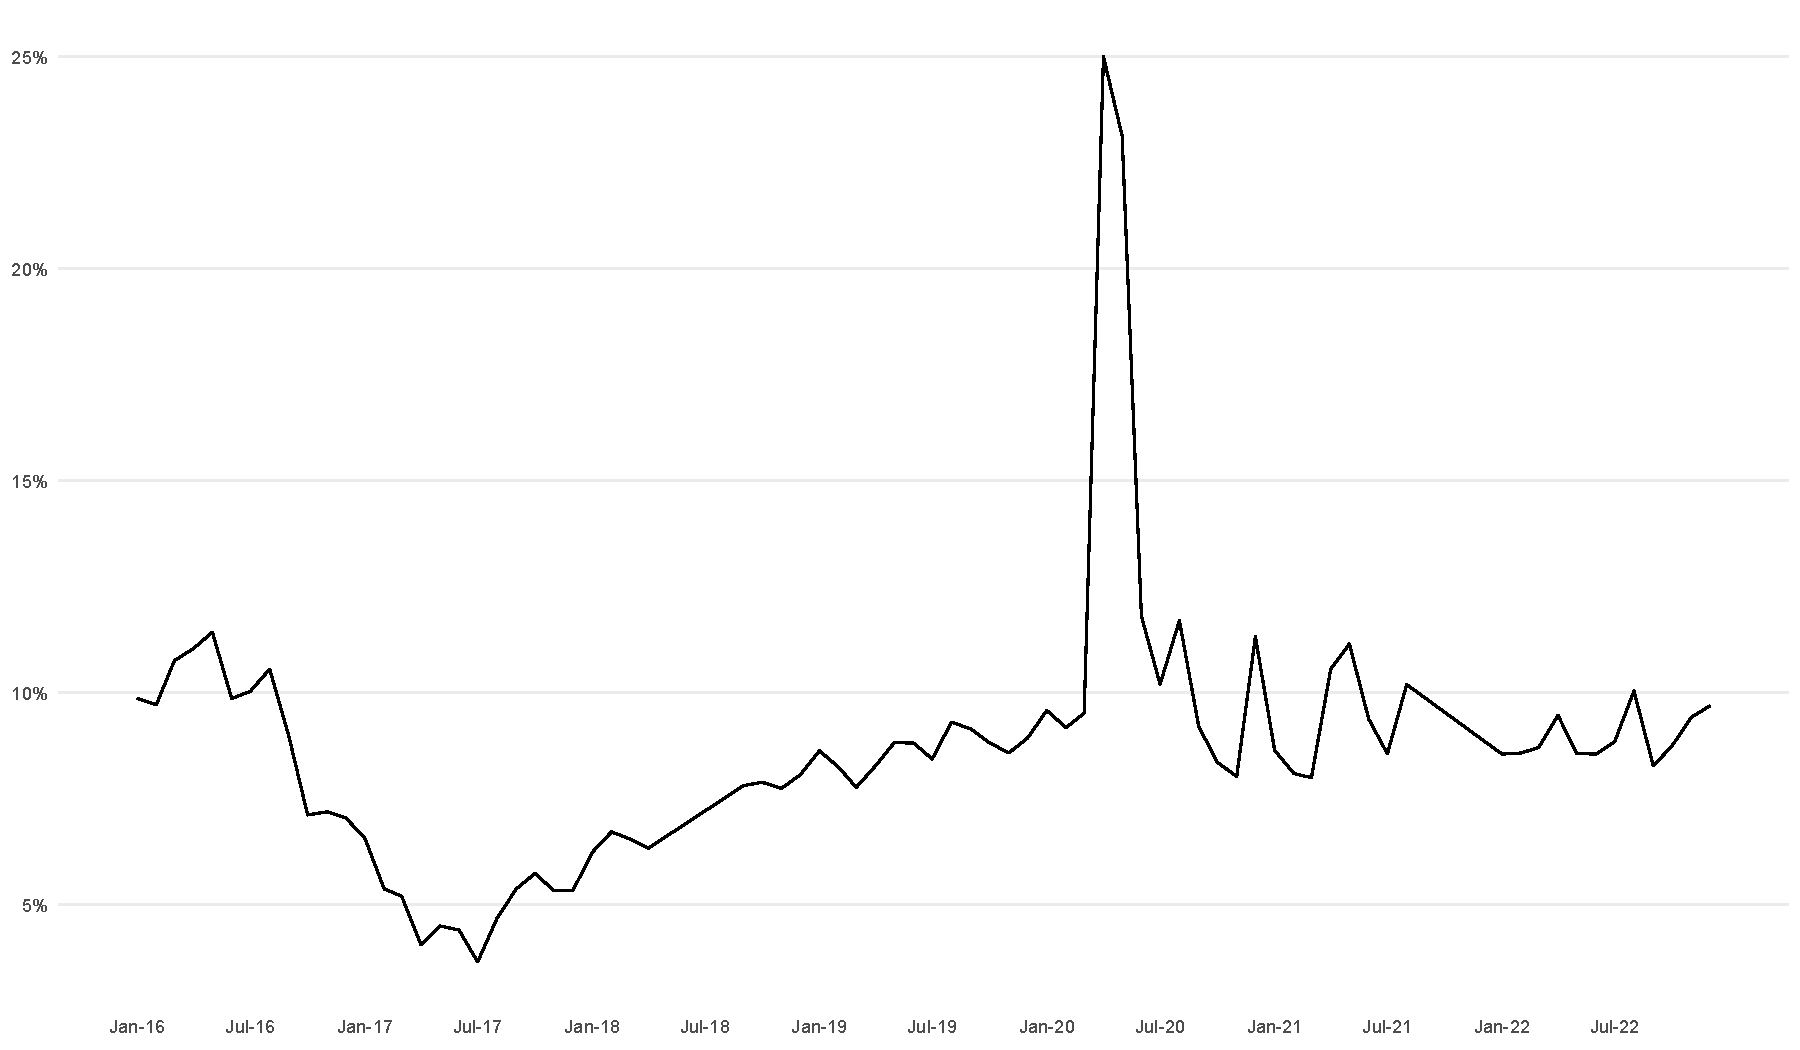
\includegraphics[width=\linewidth,height=1.5\textheight,keepaspectratio]{images/unemp_plot.pdf}

}

\caption{\label{fig-unemp}Unemployment Rate}

\end{figure}%

\FloatBarrier

sourece: '' nnnd'' \FloatBarrier

\FloatBarrier

\begin{table}

\caption{\label{tbl-correlation}Correlation Matrix}

\centering{

    \centering
    
    
    \begin{tabular}{l c c c c c}
        \toprule
        & \shortstack{Consumption \\ Growth \\ (Food Bundle)} & \shortstack{Consumption \\ Growth \\ (Food \& Fuel Bundle)} & \shortstack{Business \\ Conditions} & \shortstack{Financial \\ Position} & \shortstack{ICS} \\
        \midrule
        Business Conditions & $0.66^{***}$ & $0.59^{***}$ & -- & -- & -- \\
        Financial Position & $0.62^{***}$ & $0.54^{***}$ & $0.99^{***}$ & -- & -- \\
        ICS & $0.65^{***}$ & $0.57^{***}$ & $1^{***}$ & $1^{***}$ & -- \\
        \bottomrule
    \end{tabular}
    \caption*{\footnotesize \textbf{Note:}  ***, **, * represent significance at 1\%, 5\%, and 10\% level respectively.}

}

\end{table}%

\FloatBarrier




\end{document}
